\documentclass[12pt,a4paper]{article}
\usepackage[utf8]{inputenc}
\usepackage[german]{babel}
\usepackage{amssymb}
\usepackage{hyperref}
\usepackage{amsmath}
\usepackage{amsfonts}
\usepackage{hyperref}
\usepackage{amssymb}
\usepackage{graphicx}
\usepackage{epstopdf}
\usepackage{tabto}
\usepackage[left=2cm,right=2cm,top=2cm,bottom=2cm]{geometry}
\usepackage{listings}
\usepackage{awesomebox}

\lstset{
	language=bash,
	basicstyle=\ttfamily
}
\author{Christian Grieß}
\begin{document}
\begin{titlepage}
\begin{figure}
	\centering 
\includegraphics[scale=0.5]{./Bilder/HTWLogo/HTWD.png}
\end{figure}


	\centering
	{\scshape\LARGE Hochschule für Technik und Wirtschaft Dresden \par}
	\vspace{2cm}
	{\scshape\Large Übertragung von Sensordaten mittels LoRa\par}
	\vspace{0cm}
	{\scshape\Large Projektseminar \par}
	\vspace{1.5cm}
	{\huge\bfseries Katastrophennetz\par}
	{\huge\bfseries mithilfe von Meshtastic\par}
	\vspace{1.5cm}
	{\huge\bfseries {Dokumentation}\par}
	\vspace{4cm}
	{\Large\itshape Christian Grieß\par}
	{\Large\itshape Göran Heinemann\par}
	{\Large\itshape Julian Meinking\par}
	\vfill
	unter Aufsicht von\par %betreut von
	Prof. Dr.-Ing.~Jörg \textsc{Vogt}

	\vfill

% Bottom of the page
	{\large \today\par}
\end{titlepage}
\newpage
\tableofcontents

\newpage
\section{Aufgabenstellung}

Ziel dieses Projekts war das Experimentieren mit Meshtastic auf LoRa-fähigen Geräten.
Meshtastic ist ein Open-Source-Projekt, das es ermöglicht, ein Mesh-Netzwerk aufzubauen, das auf der LoRa-Technologie basiert.
Es ist eine kostengünstige und energieeffiziente Möglichkeit, ein Netzwerk aufzubauen, das unabhängig von Internet und
Mobilfunknetzen funktionieren kann.

\section{Fragestellung}

Ist Meshtastic als unabhängiges Kommunikations-Netzwerk für den Krisenfall im Raum Dresden geeignet?

\section{Technologie}
\subsection{Was ist LoRa?}

LoRa (von Long Range) ist eine proprietäre Funktechnologie im Besitz von Semtech. Sie ist für die Langstreckenübertragung (z.B. 10 km),
schmalbandige Übertragung (gemessen in Kbps) und energiesparende Kommunikation konzipiert, hauptsächlich für Internet of Things (IoT)-Netzwerke.
Dafür wird eine drahtlose Modulationstechnik, die aus der Chirp Spread Spectrum (CSS)-Technologie abgeleitet ist, verwendet.
Sie codiert Informationen auf Radiowellen mithilfe von Chirp-Impulsen. Die modulierte Übertragung von LoRa ist robust gegen Störungen
und kann über große Entfernungen empfangen werden.

Es eignet sich ideal für Anwendungen, die kleine Datenmengen mit niedrigen Bitraten übertragen. Daten können über eine längere Reichweite
übertragen werden im Vergleich zu Technologien wie WLAN, Bluetooth oder ZigBee. Diese Eigenschaften machen LoRa besonders geeignet für
Sensoren und Aktoren, die im Niedrigenergiemodus arbeiten.

Außerdem arbeitet LoRa in einem lizenzfreien Sub-Gigahertz-Frequenzband (d.h. unter 1 GHz), aber die zu verwendenden Frequenzen variieren
von Region zu Region aufgrund regulatorischer Anforderungen. Wenn Sie ein LoRa-Gerät kaufen, muss sichergestellt sein, dass das richtige
Frequenzband unterstützt wird.

In Europa - 863–870MHz (normalerweise 868MHz).
\newpage
\subsection{Warum LoRa?}

LoRa versucht die Lücke zwischen zwischen Kommunikationstechnologien wie WiFi, Bluetooth und LTE zu schließen.\\

\begin{figure}[h]
	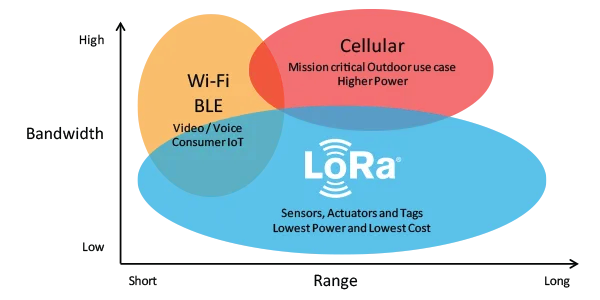
\includegraphics[scale=0.7]{./Bilder/Technologie/bandwidth-vs-range.png}
\end{figure}
\url{https://www.semtech.com/uploads/images/LoRa_Why_Range.png}\\ \\
Es ist für große Reichweite, kleine Bandbreite und Niedrigenergiekommunikation gemacht. Alles in allem also extrem nützlich für IoT Geräte.
Einige Beispiele sind:

\begin{itemize}
	\item Wassersensoren in einer entfernten Umgebung (Grundwasser)
	\item Rauchwarnmelder
	\item Tierbeobachtung
	\item Verbrauchsmessungen bei Endkunden (Gas, Strom)
	\item Wetterstationen die nur ab und zu Informationen übertragen
\end{itemize}
\newpage
\subsection{LoRa und LoRaWAN}

LoRaWAN ist über LoRa angesiedelt und definiert das Kommunikationsprotokoll und die Systemarchitektur.

Es ist wichtig zu verstehen, dass es möglich ist LoRa ohne LoRaWAN zu benutzen. Andere LoRa-basierte Netzwerke sind Helium,
The Things Network, Disaster.radio und was wir weiter betrachten werden, Meshtastic.

\subsection{Meshtastic}
Wie im vorherigen Absatz erwähnt, baut Meshtastic auf LoRa auf und schafft ein dezentralisiertes Mesh-Netzwerk.

Es bringt folgende Eigenschaften mit sich:
\begin{itemize}
	\item Verschlüsselte und Textbasierte Kommunikation
	\item Plattformunabhängig
	\begin{itemize}
		\item Computer (unabhänging vom Betriebssystem)
		\item Android (native App)
		\item iOS (native App)
	\end{itemize}
	\item Dezentralisiert
	\item Geringer Stromverbrauch
	\item Optionales Standort teilen
	\item Open-Source
\end{itemize}

Anders als traditionelle Mobilfunknetzwerke, verbindet sich jedes Endnutzergerät mit einem LoRa Radio
und alle LoRa Radios, welche Meshtastic nutzen, können Nachrichten, selbst wenn die Radios nicht im gleichen Mesh sind, weiterleiten.
Das passiert so lange, bis die Nachricht Ihr Ziel erreicht oder die voreingestellten “Hops” ausgeschöpft werden.

\begin{figure}[h]
	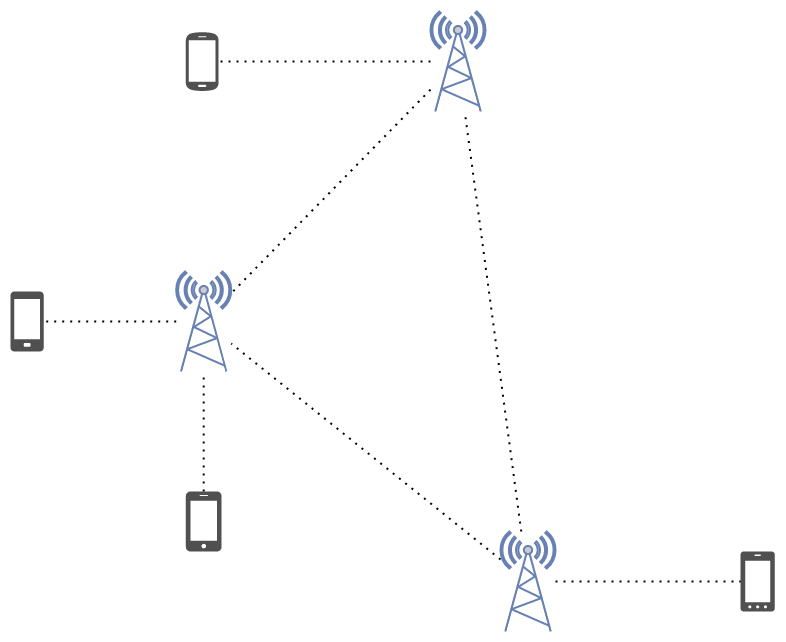
\includegraphics[scale=0.4]{./Bilder/Technologie/meshtastic-connections.png}
\end{figure}

\url{https://loganmarchione.com/2023/05/lora-and-meshtastic/20230510_003.png}

\newpage

\section{Geräte}

Folgende Geräte haben wir für das Projekt genutzt:

\subsection{Heltec LoRa32 v3}

max TX power: +21dBm\\
\begin{figure}[h]
	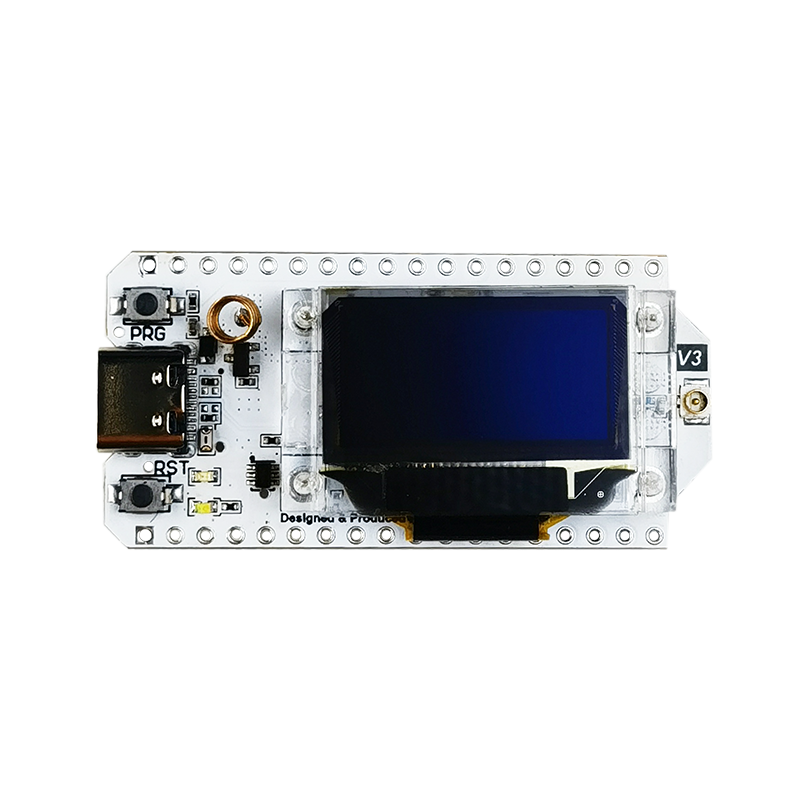
\includegraphics[scale=0.1]{./Bilder/Devices/heltec-lora32-v3.png}
\end{figure}\\
\url{https://heltec.org/project/wifi-lora-32-v3}\\

\subsection{LILYGO T-Echo}
max TX power: +21dBm\\
\begin{figure}[h]
	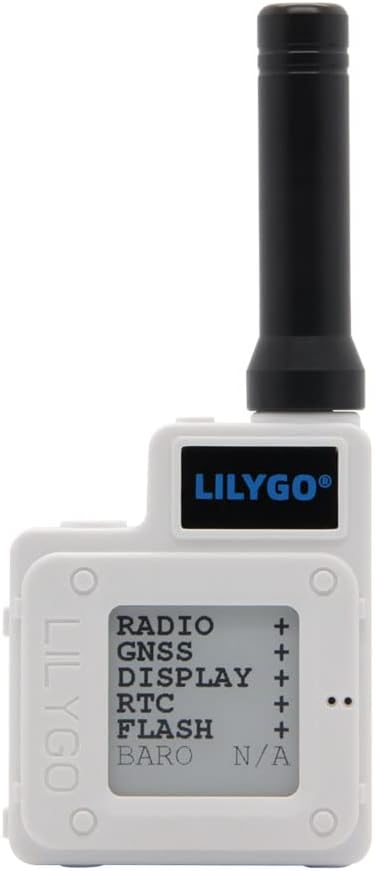
\includegraphics[scale=0.1]{./Bilder/Devices/t-echo.jpg}
\end{figure}\\
\url{https://www.lilygo.cc/products/t-echo}\\

\subsection{LILYGO T-Deck}
max TX power: +21dBm\\
\begin{figure}[h]
	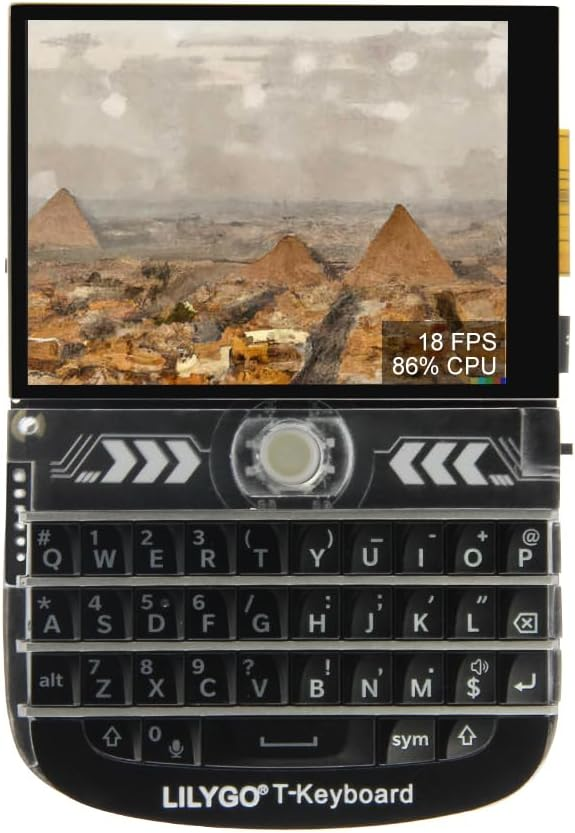
\includegraphics[scale=0.1]{./Bilder/Devices/t-deck.jpg}
\end{figure}\\
\url{https://www.lilygo.cc/products/t-deck}
\newpage
\section{Firmware flashen}

Meshtastic bietet eine Firmware für verschiede Geräte an. Je nach Gerät gibt es kleine Unterschiede
in Funktionalität (Display-Support, Speicher, etc.) und im Flashvorgang.

\subsection{Hardware identifizieren oder auswählen}
\warningbox{Achtung! Vorweg, Geräte nur mit angeschlossener Antenne einschalten! Anderenfalls kann das Gerät sich im schlimmsten Fall selber zerstören.}

Meshtastic wird offiziell nur von bestimmten Geräten unterstützt, welche ein LoRa Modul besitzen.
\\
Es ist darauf zu achten, dass jedes Gerät welches im Meshnetz betrieben werden soll, auf der gleichen Frequenz arbeitet. Hier gibt es Unterschiede!\\
\\
In Deutschland können die freien Frequenzbänder 433 MHz und 868MHz, auf welchen Lora operiert, ohne Lizenzkosten oder Amateurfunklizenz genutzt werden.\\
\\
Solange eine WLAN-Verbindung zu einem Device nicht notwendig ist und Bluetooth ausreicht, sollte ein nRF52 Chip gewählt werden,
da diese energieffizienter als ESP32 Chips und einfacher zu flashen sind. Es gibt auch noch Geräte auf Basis des RP2040,
diese haben wir allerdings nicht getestet.\\
\\
Eine Liste mit unterstützer Hardware findet sich hier:\\
\url{https://meshtastic.org/docs/hardware/devices/}

\subsubsection{Serial Treiber für ESP32}
Einen für das eigene Betriebssystem passenden Treiber auf folgender Seite identifizieren, herunterladen und Installieren:
\\
\url{https://meshtastic.org/docs/getting-started/serial-drivers}

\subsubsection{Serial Treiber für nRF52}
nRF52 Chips benötigen normalerweise keinen Serial Treiber. Sie benutzen einen UF2 bootloader, welche das Gerät als USB-Stick vom Betriebssystem erkennen lassen.

Auf keinen Fall folgenden USB geräte treiber herunterladen, es sei denn es wird UF2 support benötigt

\url{https://meshtastic.org/docs/getting-started/serial-drivers/nrf52}

\subsection{Firmware für ESP32 flashen}
\url{https://meshtastic.org/docs/getting-started/flashing-firmware/esp32/}
\\
Da es bei uns auf verschieden PCs Probleme gab haben wir zum Flashen unter Linux eine \href{https://github.com/go3ranh/meshtastic-flasher}{Nix-Flake} erstellt,
die Python mit den richtigen Paketen installiert und eine kleine Anleitung (auch zum selber Compilieren der Firmware)
für ESP32 und nRF52 Geräte enthält.\\

\subsection{Firmware für ESP32 nRF52}
\url{https://meshtastic.org/docs/getting-started/flashing-firmware/nrf52/}
\\
Beim diesen Geräten ist es bei uns manchmal vorgekommen, dass das Flashen von Firmware zwar bis zu dem “Drag und Drop”-Schritt funktioniert und dann aber nicht wirklich mit der neuen Version neu startet. Falls das passiert muss man sich mit einer seriellen Konsole mit dem Gerät verbinden und einfach nur einmal Enter drücken, besonders nachdem Factory-Erase. Das steht unter dem Punkt Factory-Erase auch dokumentiert, aber man benötigt nicht zwingend die Meshtastic CLI, sondern lediglich ein Programm wie z. B. minicom unter Linux.

\section{Software}

Zum aktuellen Zeitpunkt gibts es jeweils eine App für iOS und Android. Außerdem gibt es einen Web Client,
der sich per Bluetooth, Wi-Fi und Serial verbinden kann.\\

\begin{tabular}[h]{l | l | l}
App & Link & Quellcode \\

\hline
Android  & \href{https://play.google.com/store/apps/details?id=com.geeksville.mesh}{Playstore} & \href{https://github.com/meshtastic/Meshtastic-Android}{Github} \\
\hline
iOS & \href{https://apps.apple.com/us/app/meshtastic/id1586432531}{App Store} & \href{https://github.com/meshtastic/Meshtastic-Apple}{Github}  \\
\hline
Web & \href{https://client.meshtastic.org/}{Web App} & \href{https://github.com/meshtastic/web}{Github} \\
\end{tabular}\\
\\

Die Apps werden regelmäßig geupdated und sind modern aufgebaut.\\ \\
Ursprünglich sollte hier ein Vergleich der Funktionalitäten erfolgen, es gibt aber keine erkennbaren Unterschiede, außer kleinere in der Bennennung und Bedienung.\\

\subsection{UI}
\subsubsection{iOS}
\begin{tabular}[h]{l  l  l}
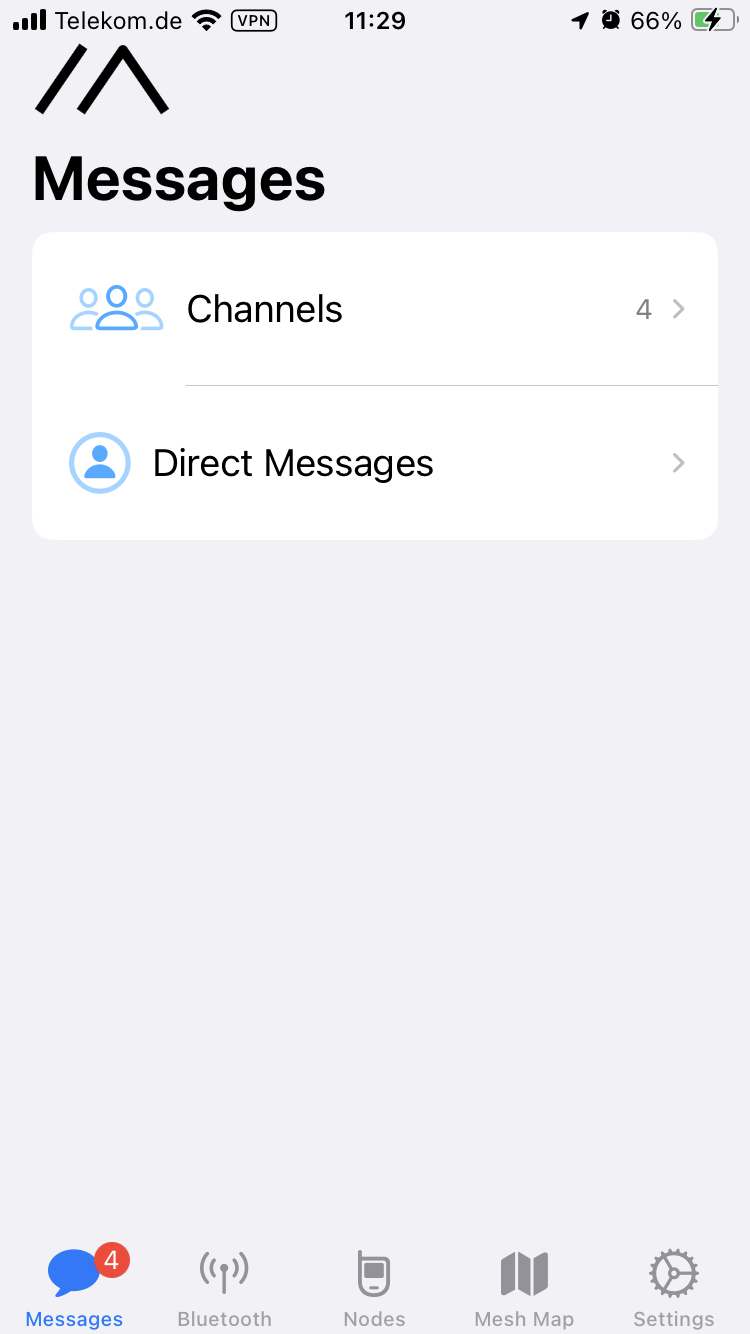
\includegraphics[scale=0.2]{./Bilder/Software/ios/messages.png} & 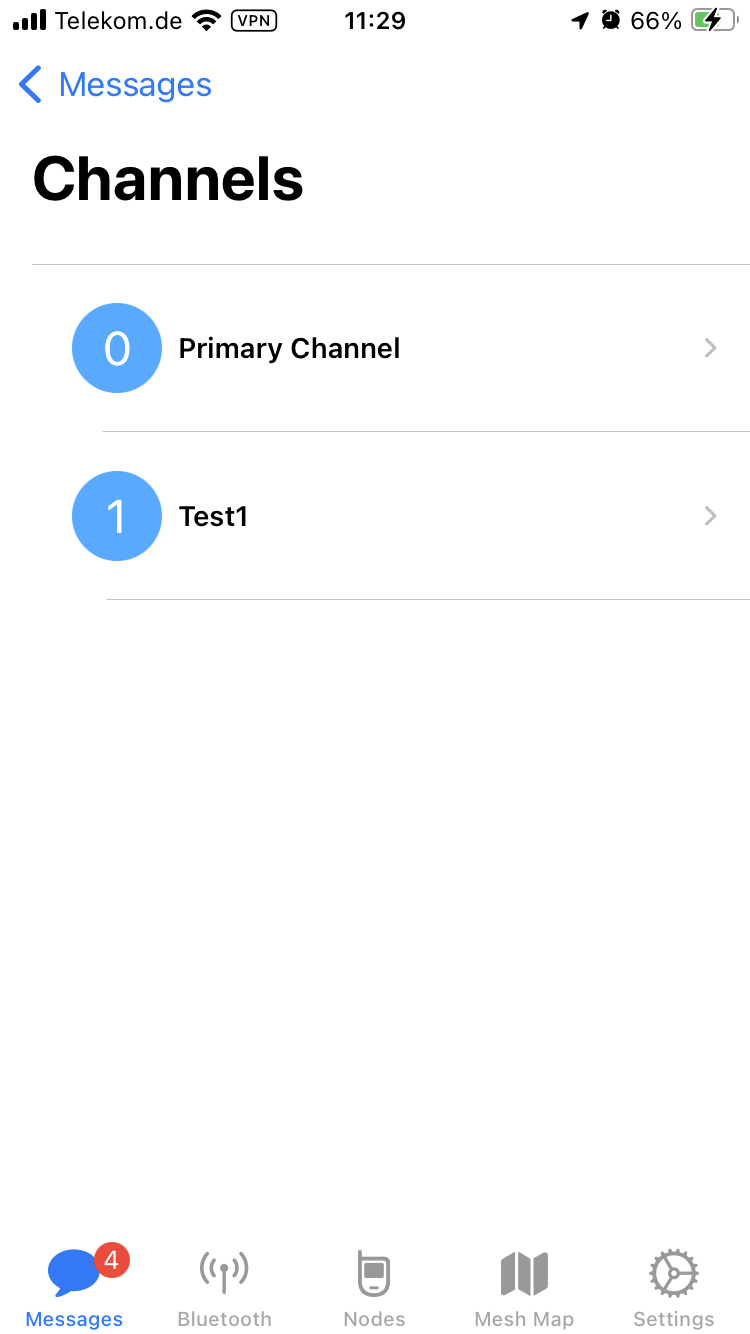
\includegraphics[scale=0.2]{./Bilder/Software/ios/messages_channels.png} & 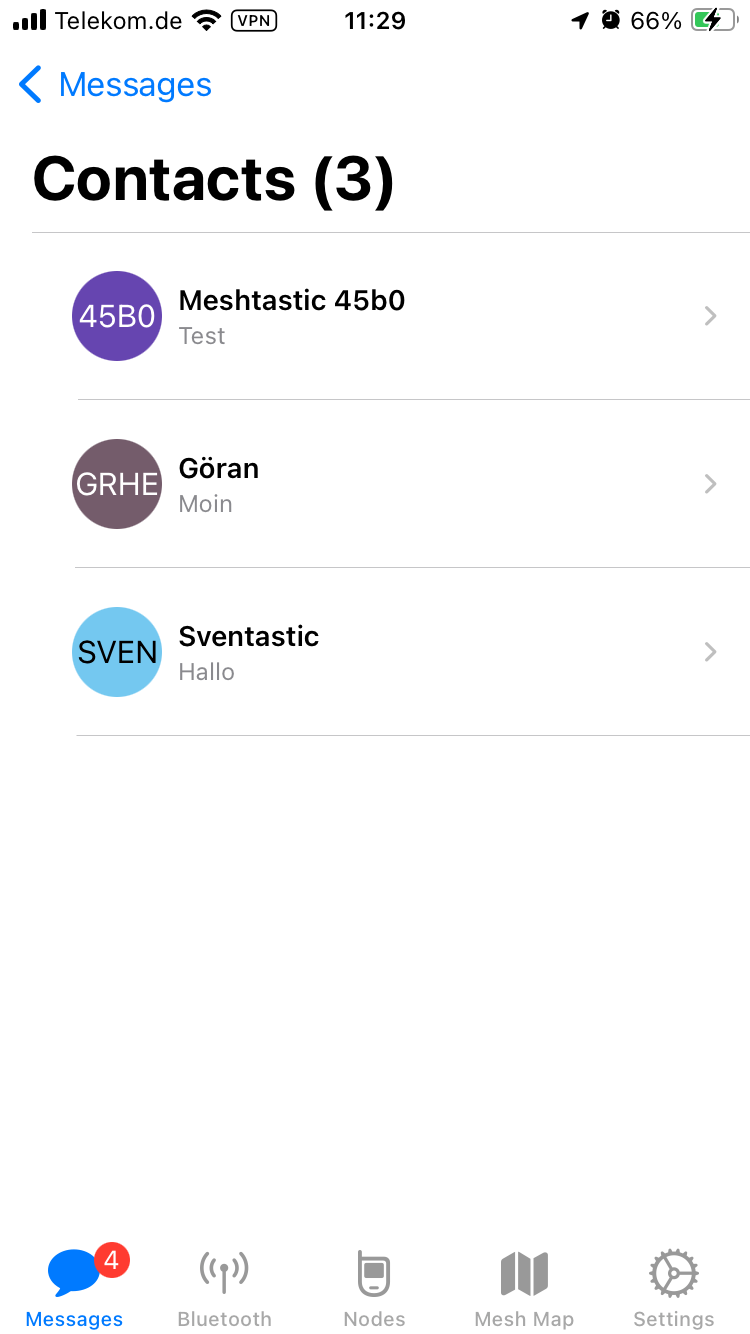
\includegraphics[scale=0.2]{./Bilder/Software/ios/messages_contacts.png}\\
Nachrichten Tab & Nachrichten in Channels & Direktnachrichten mit \\
 & & anderen Nodes\\
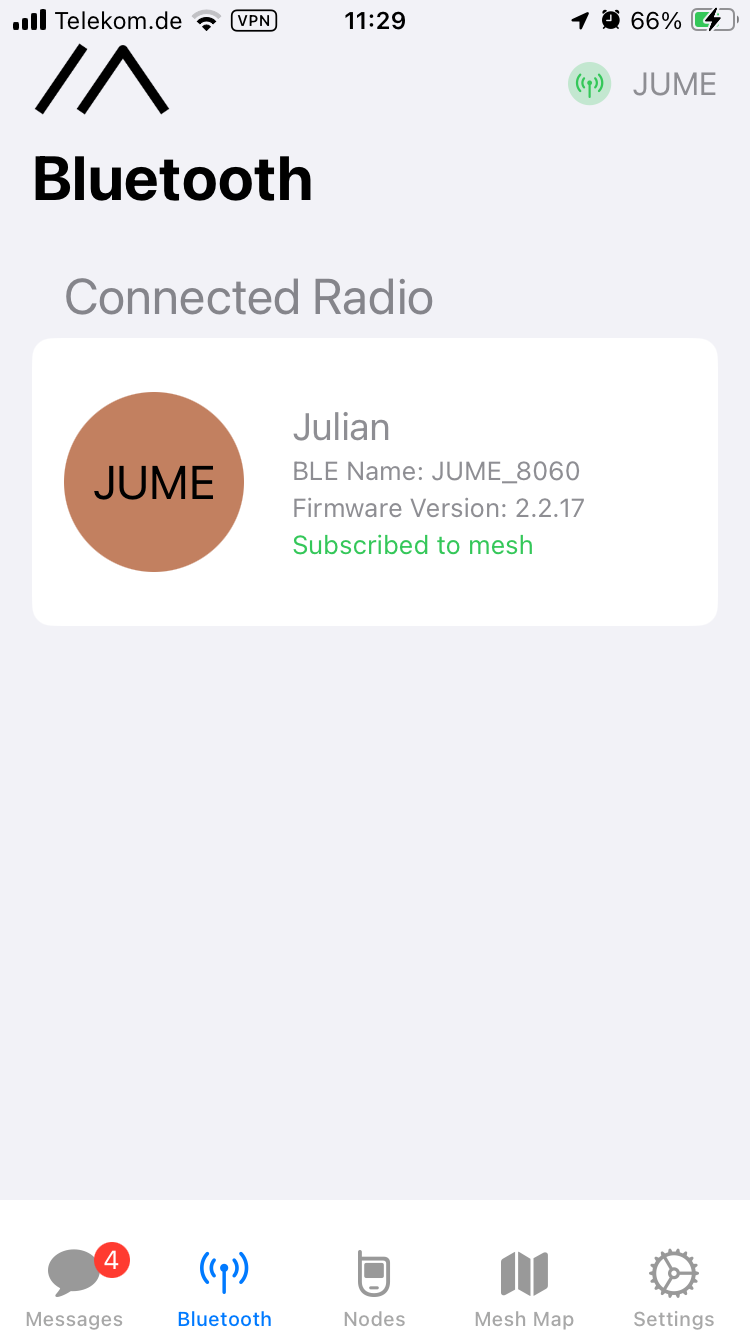
\includegraphics[scale=0.2]{./Bilder/Software/ios/bluetooth.png} & 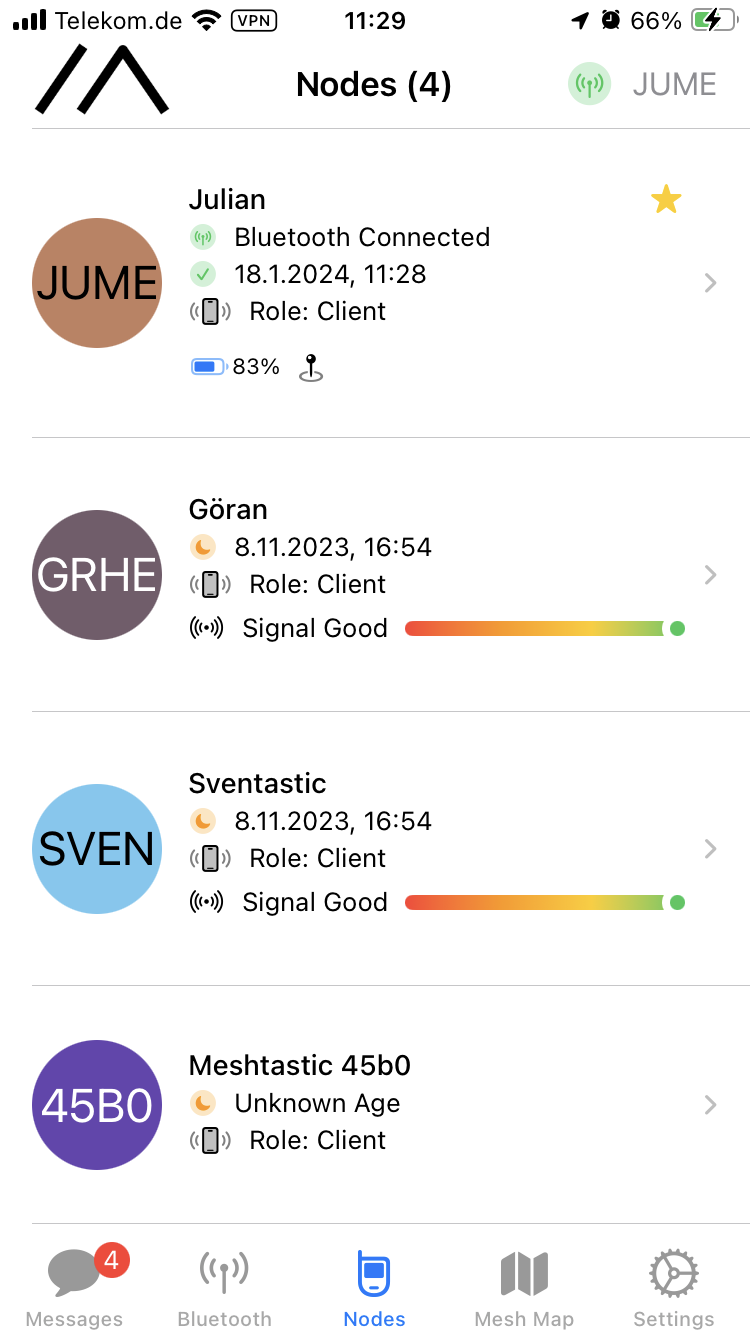
\includegraphics[scale=0.2]{./Bilder/Software/ios/nodes.png} & 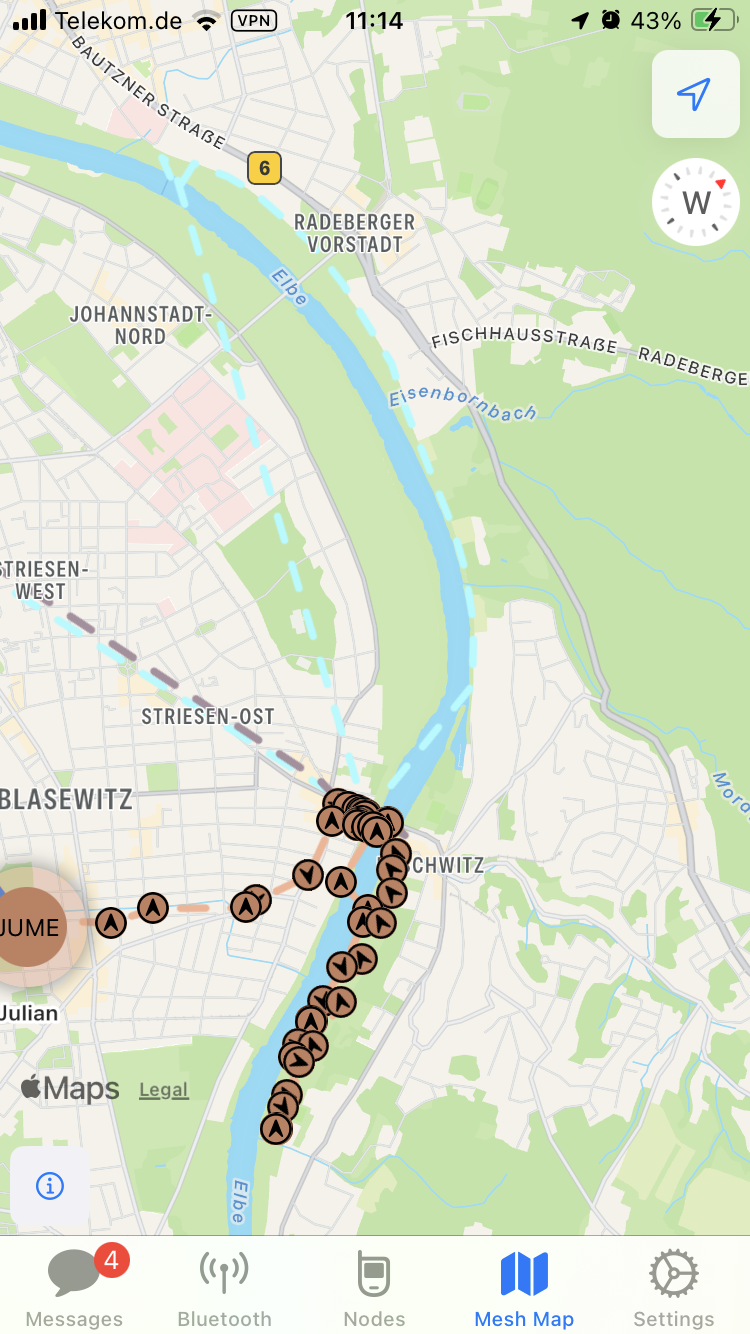
\includegraphics[scale=0.2]{./Bilder/Software/ios/mesh_map.png}\\
Bluetooth-Verbindung zum & Übersicht der verbundenen & Kartenansicht \\
eigenen Node  & Nodes \\
\end{tabular}\\
\begin{tabular}[h]{l  l}
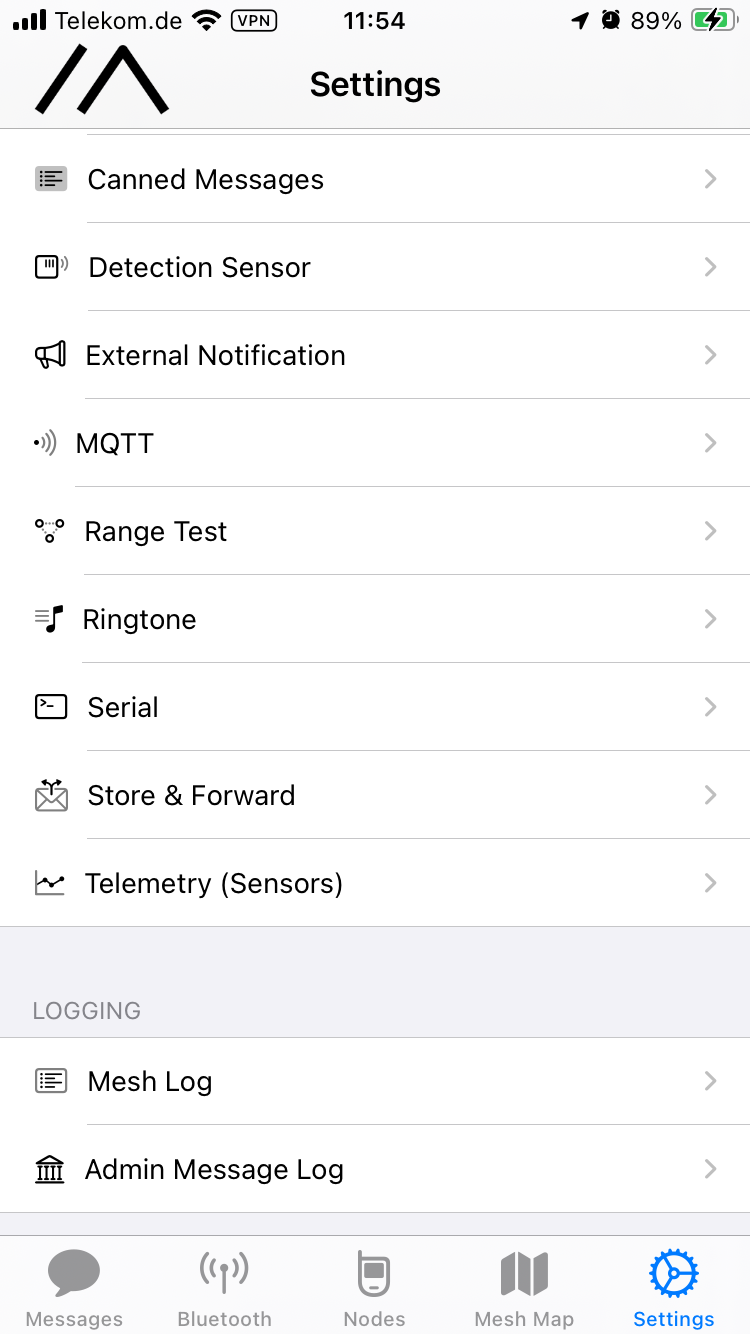
\includegraphics[scale=0.2]{./Bilder/Software/ios/config_module.png} & 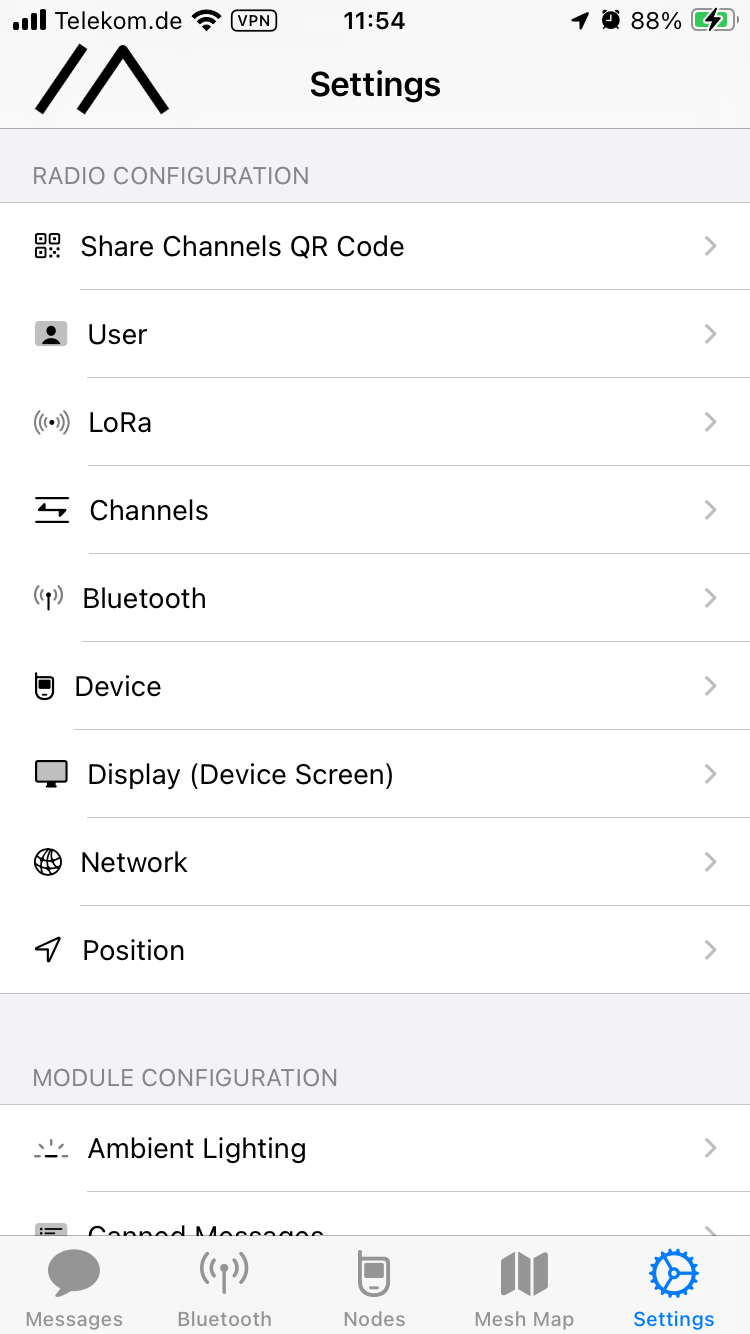
\includegraphics[scale=0.2]{./Bilder/Software/ios/config_radio.png}  \\
Modul-Konfiguration & Radio-Konfiguration\\
\end{tabular}\\

\subsubsection{Web}

\begin{tabular}[h]{l }
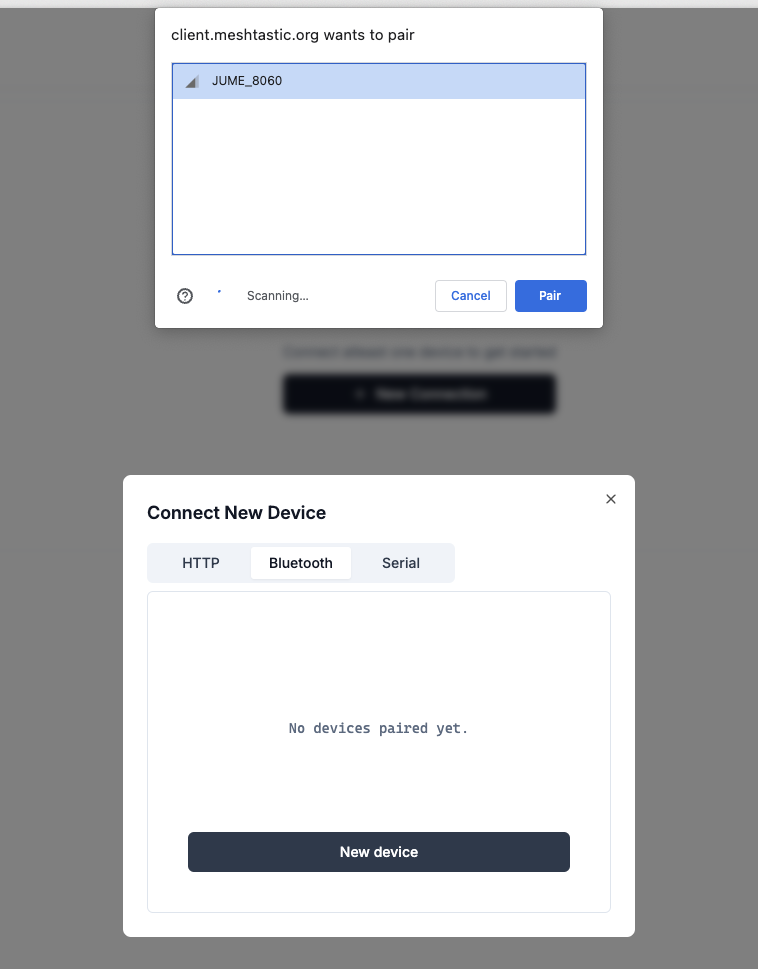
\includegraphics[scale=0.2]{./Bilder/Software/web/connection_bluetooth.png}  \\
Blluetooth-Verbindung mit Node
\end{tabular}\\
\begin{tabular}[h]{l l}
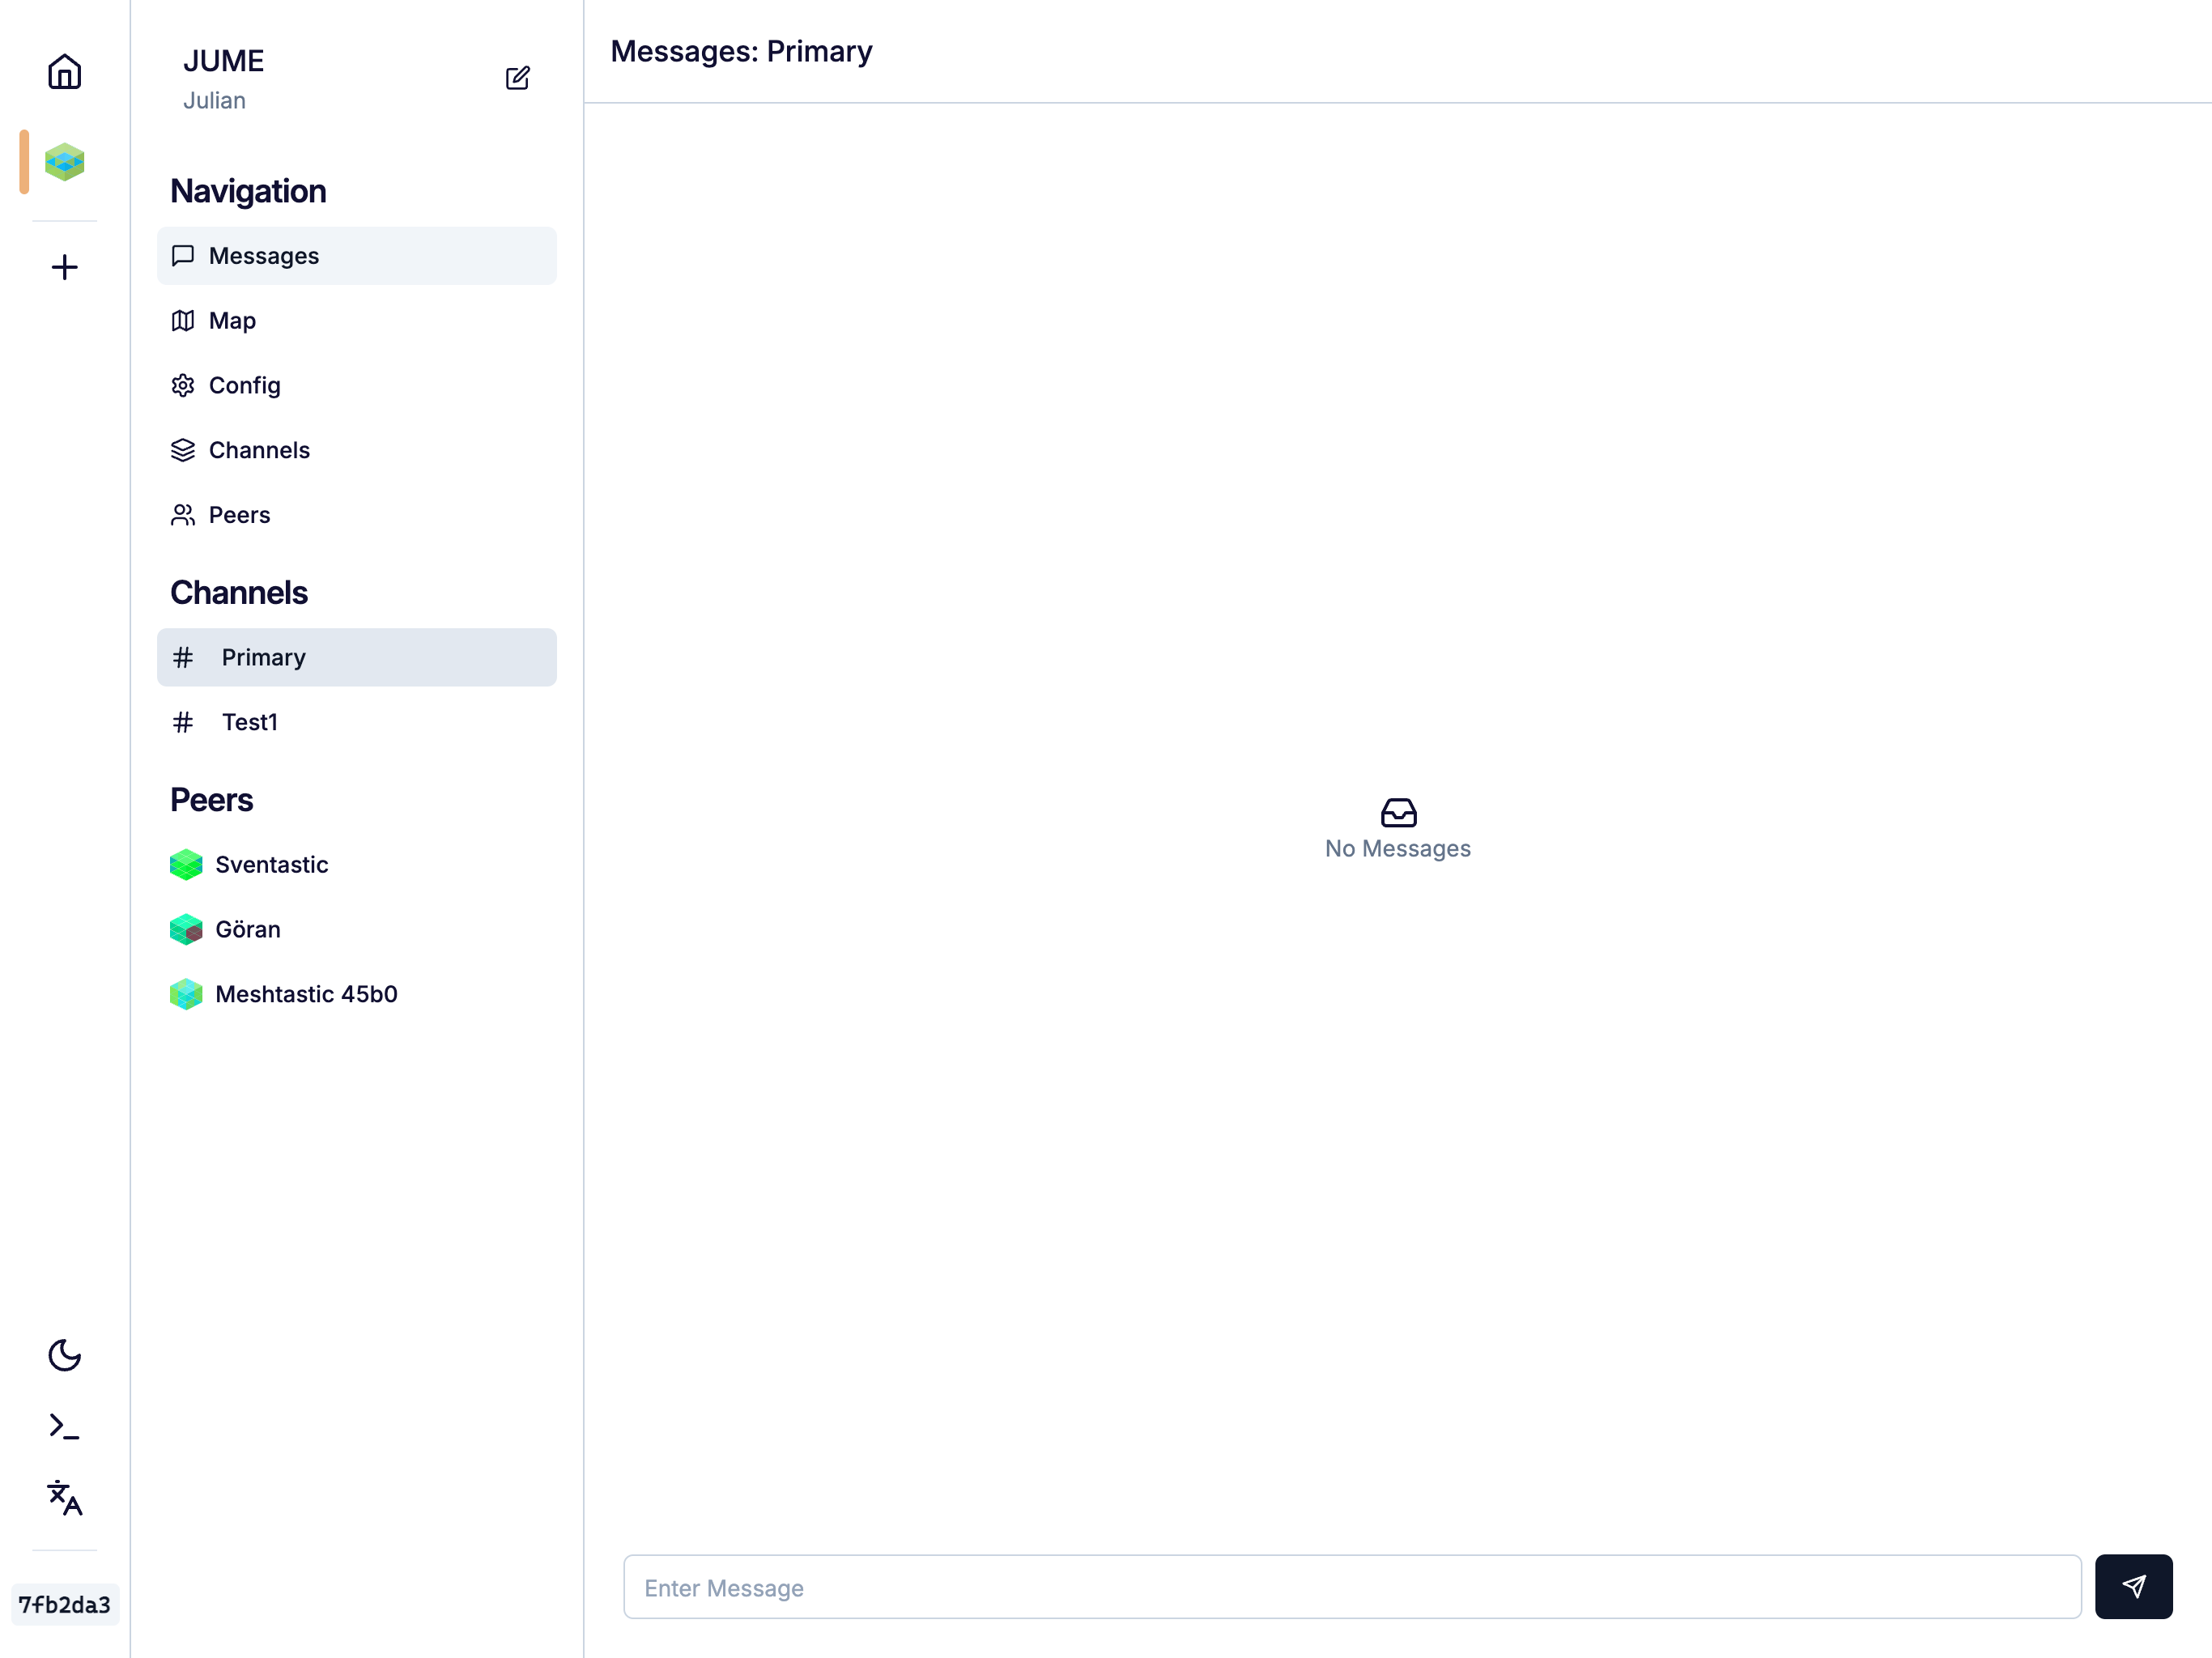
\includegraphics[scale=0.08]{./Bilder/Software/web/messages.png} & 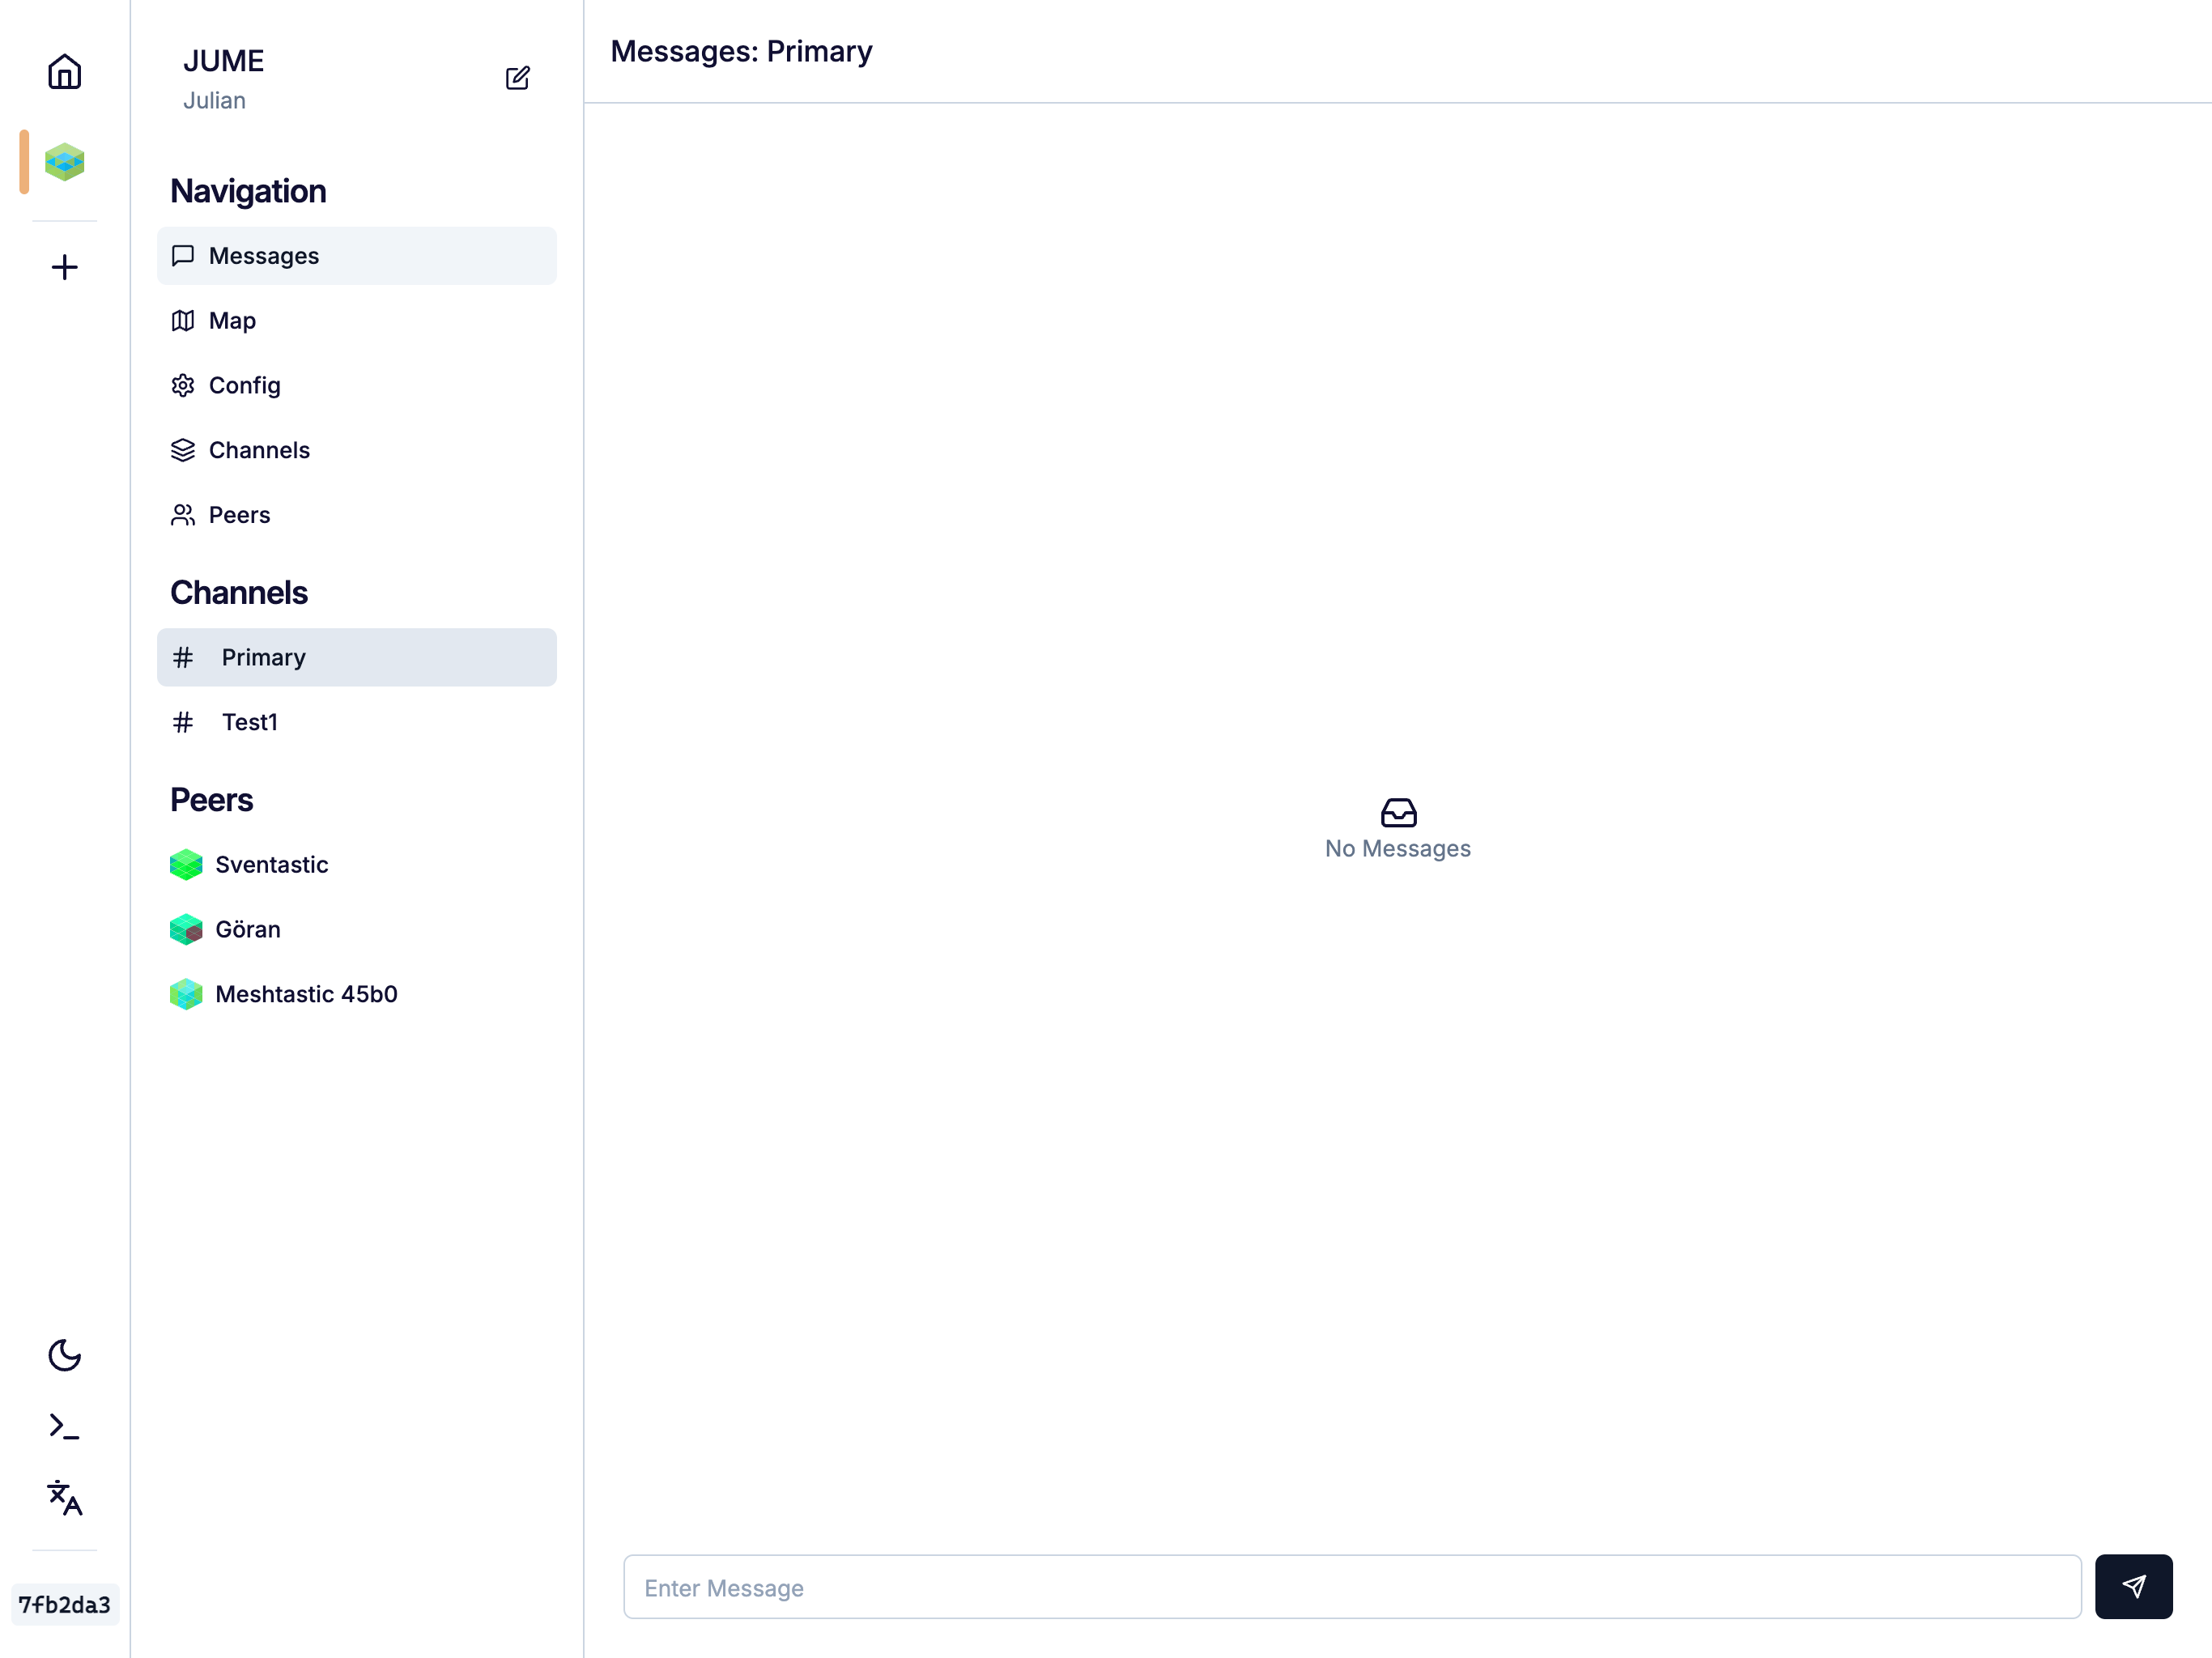
\includegraphics[scale=0.08]{./Bilder/Software/web/messages.png}\\
Nachrichten & Übersicht der Verbundenen Nodes\\
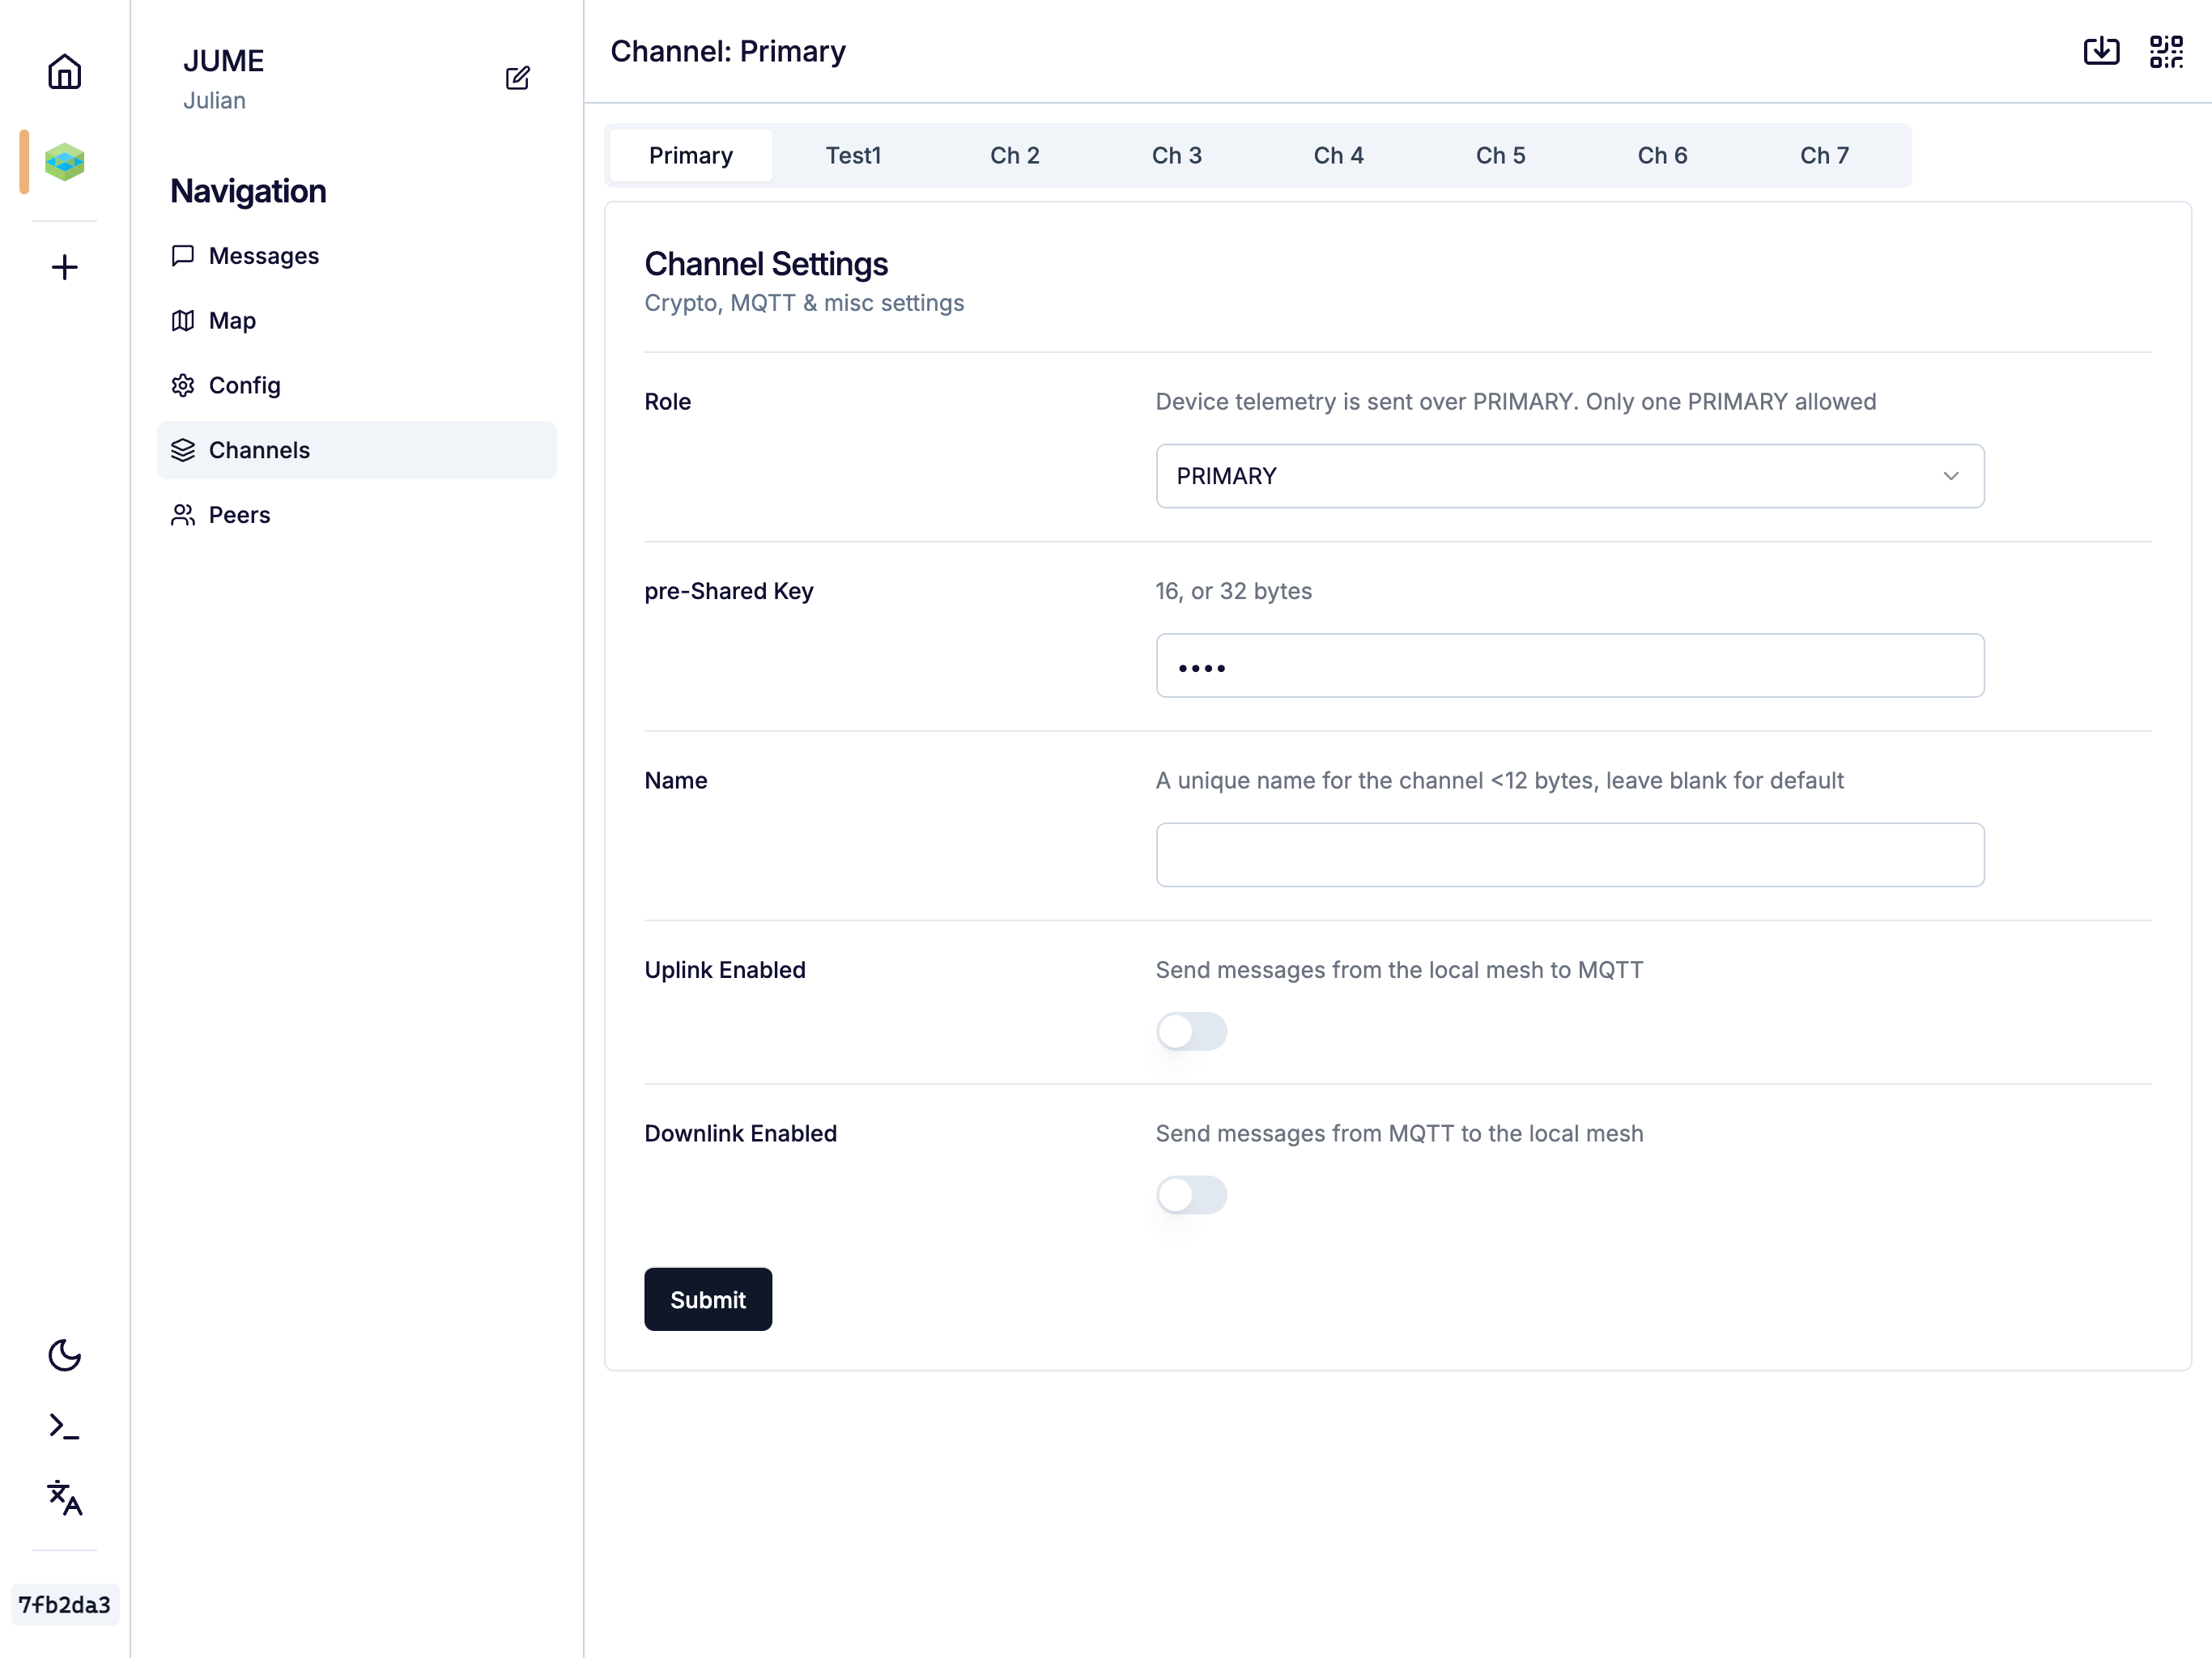
\includegraphics[scale=0.08]{./Bilder/Software/web/config_channels.png} & 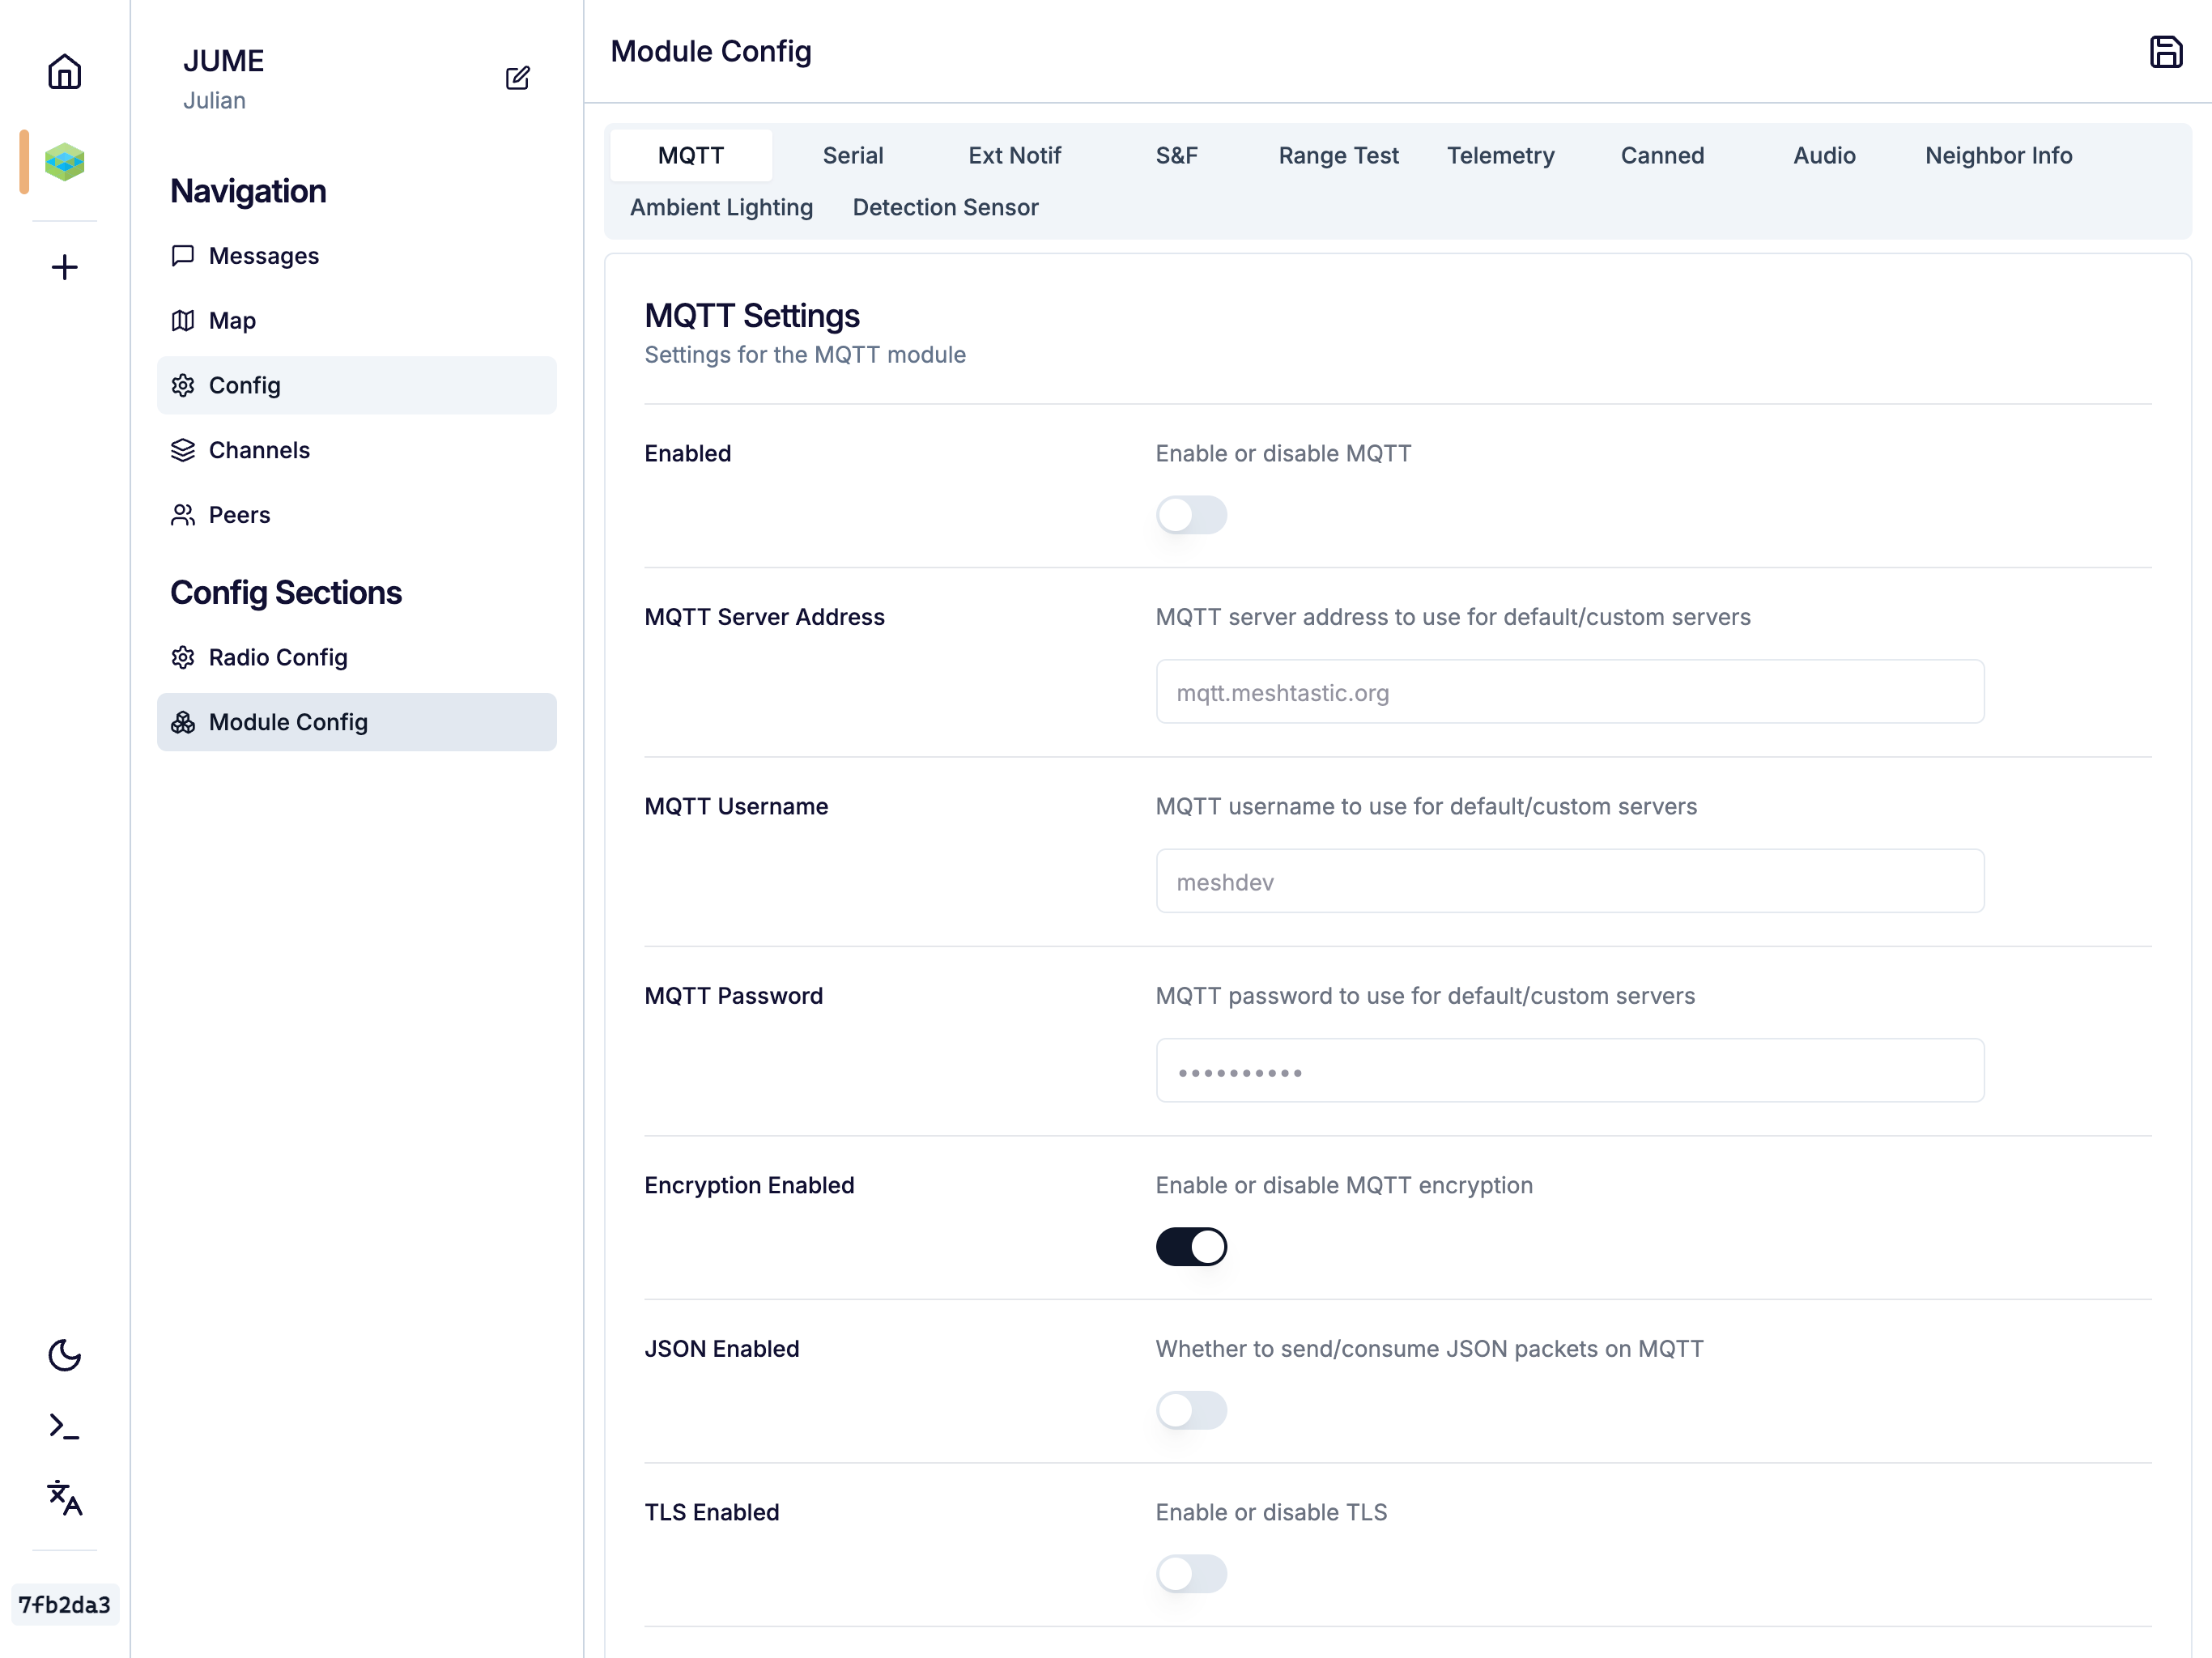
\includegraphics[scale=0.08]{./Bilder/Software/web/config_module.png}\\
Channel-Konfiguration & Modul-Konfiguration\\
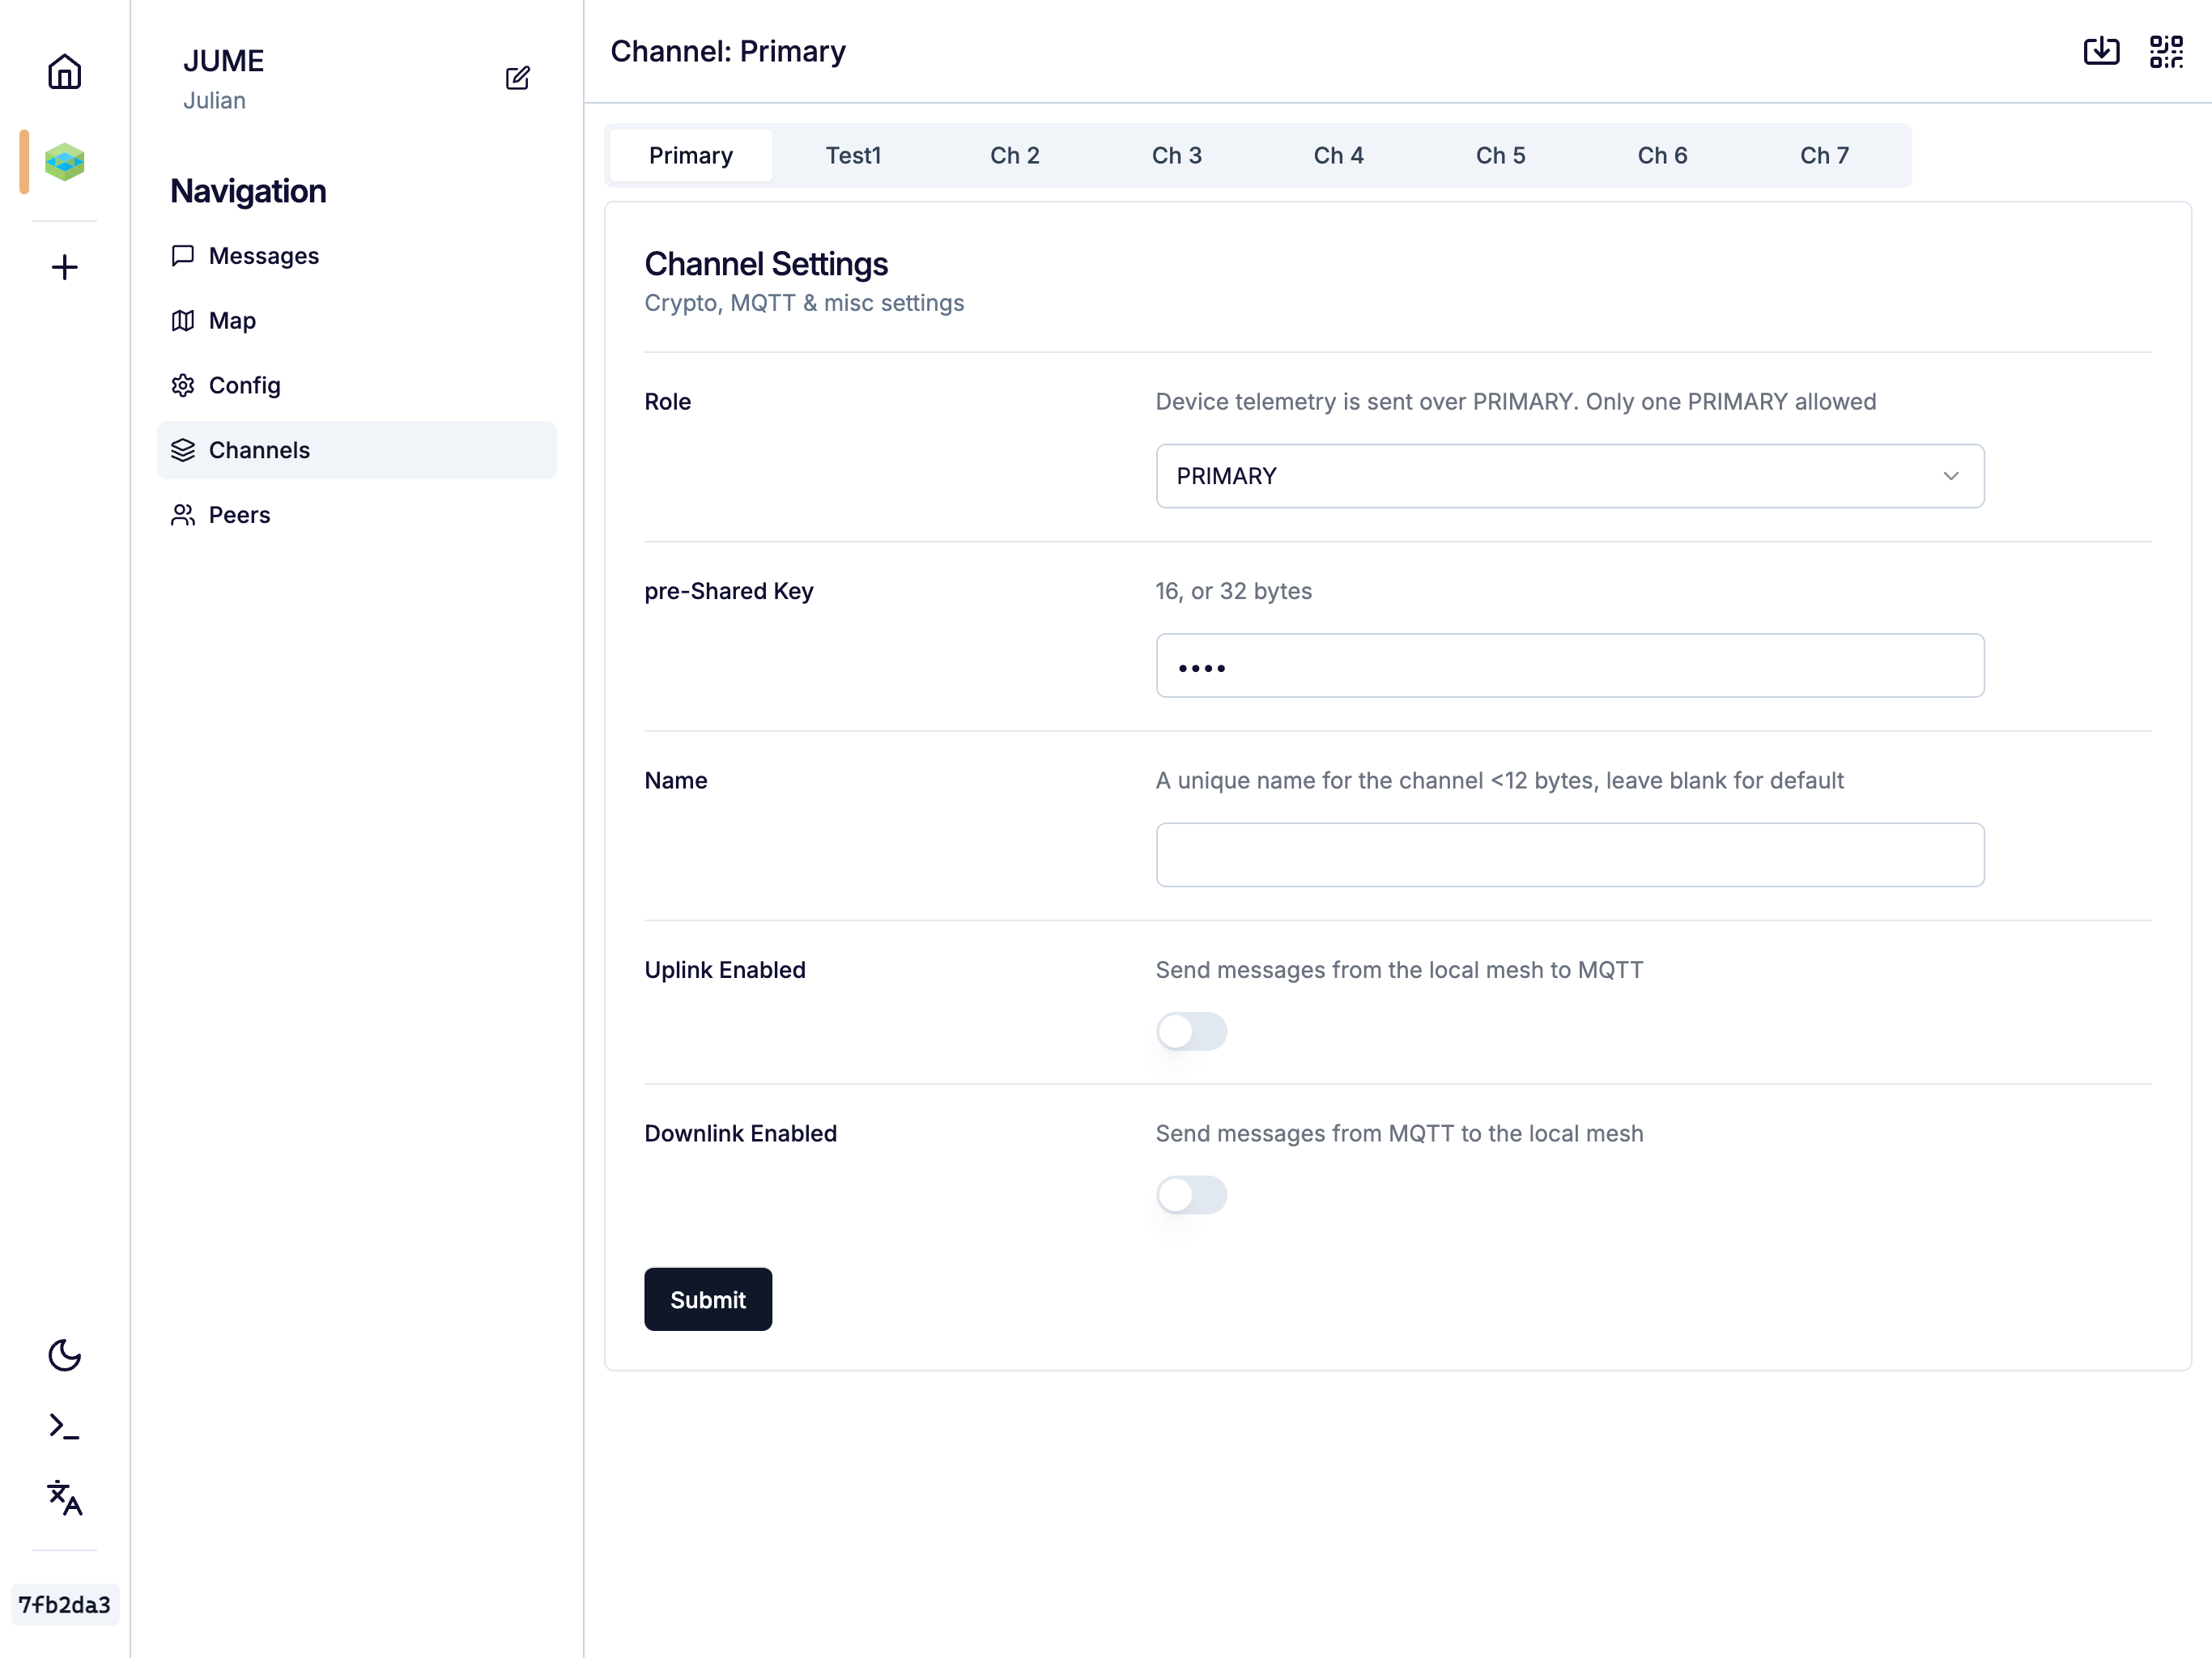
\includegraphics[scale=0.08]{./Bilder/Software/web/config_channels.png} & \\
Radio-Konfiguration
\end{tabular}\\
\section{Häufige Probleme - Kommunikation mit Gerät über USB}
\begin{itemize}
	\item Die Gerät-Datei /dev/ttyUSB0 gehört der Nutzergruppe dialout. Damit der Nutzer Schreibrechte erhalten kann, muss er zur Gruppe hinzugefügt werden:

	\lstinline{sudo usermod -aG dialout <user-name>}\\
	\lstinline{logout}

	Der Nutzer muss sich ausloggen und wieder einloggen, damit er in der Gruppe enthalten ist.
	\item Prüfen, ob das Kabel zwischen Computer und Gerät auch wirklich Daten übertragen kann.
	\item USB-C → USB-C funktioniert manchmal nicht. Dies könnte an einem Fehler bei USB-C Power Delivery liegen. Adapter USB-C → USB-A (findet man meist als OTG-Adapter) schafft Abhilfe.
\end{itemize}
\newpage
\section{Simulation}
Die Wartung vieler Meshtastic Nodes für den Zweck des Experimentierens mit der Software bzw. dem Protokoll kommt mit einem größeren Aufwand einher. Dafür kann sich eine Simulation besser eignen, um Resultate ohne Aufwand direkt beobachten zu können.

Mit der Software \href{https://github.com/GUVWAF/Meshtasticator}{Meshtasticator} ist es möglich, ein Meshtastic Netzwerk zu simulieren. Diese basiert auf zwei vorherigen Simulatoren (\href{https://github.com/lucagioacchini/lora-network-simulator}{lora-network-simulator} und \href{https://mcbor.github.io/lorasim/}{LoRaSim}) und nutzt unterliegend die \href{https://meshtastic.org/docs/software/linux-native/}{Meshtastic Linux Anwendung}, weswegen die Verwendung eines Linux Betriebsystems Voraussetzung ist.

Wir haben den Simulator in einer Ubuntu-VM installiert. Einige Pakete mussten installiert werden.
\begin{lstlisting}
	sudo apt install git python3-tk python3-pip \
	python3-venv gpiod libgpiod gpiod libgpiod-dev \
	libgpiod2 libyaml-cpp-dev libbluetooth-dev
\end{lstlisting}

Danach muss das \href{https://github.com/GUVWAF/Meshtasticator}{Meshtasticator} und \href{https://github.com/meshtastic/firmware}{Meshtastic-Firmware} Repository herunter geladen werden.

Um die Firmware zu compilieren, benötigt man PlatformIO. Das Tool lässt sich mit dem System Paketmanager wie z.B. apt installieren, häufig bekommt man eine veraltete Version, da die Paketquellen der meisten Betriebsysteme nur langsam aktualisiert werden.

Deshalb empfehlen wir, den Paketmanager von Python zu nutzen:
\begin{lstlisting}
	pip install platformio
\end{lstlisting}

Der Installationspfad liegt in ~/.local/bin, welcher nicht standardmäßig in der Systemvariable PATH enthalten sein kann. Falls der Befehl pio beim Aufruf nicht gefunden wird, reicht es aus, den Installiationspfad zum System-PATH hinzuzufügen:
\begin{lstlisting}
	export PATH="$HOME/.local/bin:$PATH"
\end{lstlisting}

Die Meshtastic Firmware, welche normalerweise für IoT Hardware kompiliert wird, kann auch nativ auf einem Linux Betriebsystem mithilfe von \href{https://github.com/meshtastic/framework-portduino}{Portduino} ausgeführt werden.

Mit Environment-Parameter native baut PlatformIO die Firmware für ein Linux Betriebsystem.
\begin{lstlisting}
	pio run --environment native
\end{lstlisting}

\tipbox{Die PlatformIO Extension für VSCode bietet eine praktische GUI, mit der die Befehle ausgeführt werden können.}

Das kompilierte Binary befindet sich dann im Ordner \lstinline{firmware/.pio/build/native}.
Damit der Meshtasticator die gewünschten Anordnungen simulieren kann, muss die Binary in den Ordner von Meshtasticator kopiert werden. Bevor die Abhängigkeiten von Meshtasticator installiert werden können, sollte in dem Ordner eine Python-Umgebung aktiviert werden:
\begin{lstlisting}
	python3 -m venv venv
	source venv/bin/activate
\end{lstlisting}
Die Abhängigkeiten können mit \lstinline{pip3 install -r requirements.txt} installiert werden.

\newpage
\section{Praxistest}

In unseren Praxistests am Elbufer in Dresden haben wir eine Reichweite von 4km Luftlinie erreicht.

Wir sind mit dem Fahrrad jeweils vom Blauen Wunder in beide Richtungen gefahren und haben unsere
Meshtastic Geräte im Rucksack mitgenommen.

Für den kontinierlichen Sendetest, haben wir in den Moduleinstellungen den Range Test aktiviert
und auf ein Interval von 1min gestellt.

\subsection{Logfiles}
\begin{tabular}[h]{l | l | l}
Node & Typ & Link \\
\hline

Göran & Metrics & \href{https://htwdd-rn.github.io/lora-meshtastic/logs/goeran%20Device%20Metrics%20Log.csv}{Download} \\
  		& Position & \href{https://htwdd-rn.github.io/lora-meshtastic/logs/goeran%20Position%20Log.csv}{Download} \\
\hline
Julian & Metrics & \href{https://htwdd-rn.github.io/lora-meshtastic/logs/Julian%20Device%20Metrics%20Log.csv}{Download} \\
			& Position & \href{https://htwdd-rn.github.io/lora-meshtastic/logs/Julian%20Position%20Log.csv}{Download} \\
\hline
Sventastic & Metrics & \href{https://htwdd-rn.github.io/lora-meshtastic/logs/Sventastic%20Device%20Metrics%20Log.csv}{Download} \\
					 & Position & \href{https://htwdd-rn.github.io/lora-meshtastic/logs/Sventastic%20Position%20Log.csv}{Download} \\
\end{tabular}\\

\subsection{Fazit}
Dieser Test konnte zeigen, dass Meshtastic mit batteriebetriebenen Geräten ohne besondere Ausrichtung
der Antennen eine gute Distanz auf Luftlinie zurücklegen kann. Wegen der Weiterleitung von Nachrichten
konnte die Verbindung zwischen Christian und Julian aufrechterhalten werden.

Die Werte ließen sich wahrscheinlich auch noch verbessern, wenn bessere Antennen verwendet würden und
eine genauere Ausrichtung der Antennen erfolgen würde.

Innerhalb der Stadt, mit vielen Gebäuden und anderen Hindernissen, ist die Reichweite wesentlich geringer.
Das Meshnetzwerk müsste dann enger aufgebaut werden, um eine gute Verbindung zu gewährleisten.

\newpage
\section{Theorie}

\subsection{Link-Budget}

Die Reichweite einer Funkverbindung lässt sich mittel des Link-Budgets (Leistungs-übertragungsbilanz)
darstellen und gibt die Qualität eines Funk-Übertragungskanals an.
Eines der einfachsten Modelle um ein Linkbudget zu errechnen ist mittels Addition der Sendeleistung
(Transmitter Power, Tx), der Empfängerempfindlichkeit (Receiver Power, Rx), des Antennengewinns und der Freiraumdämpfung (Free Space Path Loss, FSPL).

\subsection{Kenngrößen}

Der Spreading Faktor und somit die Reichweite eines Senders sind von den Ausbreitungsbedingungen abhängig.
Die Empfängerempfindlichkeit hängt von Signal-Rausch-Verhältnis (SNR), Rauschfaktor (NF) und Bandbreite (BW) ab.

Die Freiraumdämpfung beeinträchtigt die Reichweite. Durch die Verdopplung der Entfernung nimmt die Freiraumdämpfung um 6 dB zu.
Reflektionen und Brechungen der Funkwellen an Hindernissen und Boden beeinflussen Signalpegel und Reichweite. Im LoRaWAN-Netzwerk befindet sich eine Seite der Funkverbindung in der Regel in Bodennähe.
Hindernisse in der ersten Fresnelzone beeinflussen den Signalpegel auf der Rx-Seite und verkürzen die Reichweite.
SF-Werte und somit die Reichweite eines Senders hängen von den Ausbreitungsbedingungen ab. LoRaWAN erlaubt mittels ADR ein automatisches Netzmanagement und regelt damit die Reichweiten der Sender.

\subsection{dB}

Die Einheit dB (Dezibel) wird im Zusammenhang mit Funkverbindungen verwendet, um die Signalstärke, Dämpfung oder Verstärkung von elektromagnetischen Signalen zu messen. dB ist eine logarithmische Einheit, die das Verhältnis zwischen zwei Größen ausdrückt. In Bezug auf Funkverbindungen sind die beiden häufigsten Anwendungen die Messung der Signalstärke und die Angabe von Dämpfung oder Verstärkung.

\begin{enumerate}
	\item \textbf{Signalstärke in dBm (Dezibel Milliwatt):}
	\begin{itemize}
		\item  dBm misst die absolute Leistung eines Signals im Vergleich zu einem Referenzwert von 1 Milliwatt.
		\item  Ein positives dBm-Wert zeigt an, dass das Signal stärker ist als 1 Milliwatt, während ein negativer Wert darauf hinweist, dass es schwächer ist.
		\item  Beispiel: Ein Signal mit -50 dBm ist stärker als ein Signal mit -60 dBm.
	\end{itemize}

	\item \textbf{Dämpfung und Verstärkung in dB:}
	\begin{itemize}
		\item dB wird auch verwendet, um die Dämpfung oder Verstärkung von Signalen in einer Leitung oder einem System auszudrücken.
		\item Eine positive dB-Angabe deutet auf Verstärkung hin, während eine negative dB-Angabe auf Dämpfung hinweist.
		\item Beispiel: Ein Verstärker, der das Signal um 20 dB verstärkt, erhöht die Signalstärke um das 100-fache.
	\end{itemize}
\end{enumerate}

Bei Funkverbindungen wird die Signalstärke oft in dBm gemessen, während Dämpfung oder Verstärkung von Antennen, Kabeln oder
Verstärkern in einfachen dB-Angaben ausgedrückt werden. Dies ermöglicht eine präzise und effektive Kommunikation über die
Leistung von Funksignalen und die Leistung von Komponenten in drahtlosen Netzwerken.

\subsection{Channelsettings}
\begin{tabular}[h]{l | l}
Channelsetting  & Long Range / Fast \\
\hline
Alt Channelname & Long Fast \\
\hline
Data Rate & 1.07 kbps (default)\\
\hline
Spreading Factor/ Symbols & 11 / 2048 \\
\hline
Coding Rate & 4/5 \\
\hline
Bandwith & 250
\end{tabular}

\subsection{Transceiverwerte}

\begin{tabular}[h]{l | l}
transmit Power  & 21dBm \\
\hline
Antenna gain & 0dBi \\
\hline
RX sensitivity & -131dBm\\
\hline
RX antenna & 0dBi \\
\hline
Linkbudget & 152dB \\
\end{tabular} \\ \\ \\
WiFi LoRa 32 v3 (SX1262 Lora Chip)\\
P(dBm) = 21dBm\\
Max Receiving sensitivity = -136dBm@SF12 BW=125KHz\\
\\
(1)\url{https://www.semtech.com/design-support/lora-calculator}

\subsection{Maximal mögliche Übertragunsstärke}
\begin{align*}
\text{Maximal 500mW ERP (2)} \\
\text{Maximal 2.15dBi Antenne (3)} \\
\\
P(dBm) &= 10 \cdot \log_{10} (P(500 \ \mathrm{mW}) \div 1 \ \mathrm{mW}) \\
&= 26.9897000434 \\
&= 27\mathrm{dBm} \\
\\
P(max)&=P(dBm)+2.15\mathrm{dBi}\\
P(max)&=29.15dBm\\
\end{align*}
(2) \url{https://www.bundesnetzagentur.de/DE/Fachthemen/Telekommunikation/Frequenzen/Grundlagen/Frequenzplan/frequenzplan-node.html}\\
(Stand März 2022) Eintrag 251004 (Frequenznutzungsbedingungen)\\
(3) \url{https://www.thethingsnetwork.org/forum/t/max-allowed-antenna-gain-for-lora/37182}\\
\newpage
\subsection{Überlegungen}

Mit einem Link Budget von 152dBm (Einstellung = long fast, mit 21dBm transmit Power und 0dBi Antenne) lässt sich unter optimalen Bedingungen(nur Freiraumdämpfung(Vakuum)) eine Distanz von mehr als 800km Überwinden.
Da dies nur unter optimalen Bedingungen möglich ist werden solche Werte natürlich nicht erreicht.\\

Im Weltraum können Funksignale tatsächlich viel weiter reisen. Unter Normalbedingungen, auf unserem Planeten spielt die Sichtlinie eine bedeutende Rolle.
Aufgrund der Tatsache, dass die Welt eine Kugel ist, ist es möglich mit 1,7m Höhe 4,7km weit zu sehen.
Da im sub-GHz Bereich eine quasioptische Ausbreitung für Radiowellen gilt, ist der Horizont auch gleichzeitig eine Begrenzung für Funksignale.\\

Im nächsten Schritt betrachten wir die Wellenausbreitung mit dem Hata-Okumura-Modell (Hata-Modell).\\

Das Hata-Modell verwendet verschiedene Begriffe in der Dämpfungsformel, um zwischen verschiedenen Typen von Landoberflächen zu unterscheiden. Es werden ländliche bis zu dicht besiedelte Regionen unterschieden.\\

Hata-Ausbreitungsformel:\\

\begin{align*}
Loss(dB) &= A + B \cdot \log_{10}{(d)} - K + C \\
A &= 69.55 + 26.16 \cdot \log_{10}{(f)} - 13.82 \cdot \log_{10}{(h_s)} \\
B &= 44.9 - 6.55 \log_{10}{(h_s)} \\ \\
d &= \text{Distanz zwischen Sender und Empfänger (km)} \\
h_s &= \text{Höhe der Senderantenne (m)} \\
h_r &= \text{Empfängerantennenhöhe (m)} \\
K &= \text{Korrekturfaktor} \\
C &= \text{Korrekturfaktor}\\
f &= \text{Übertragungsfrequenz  [MHz]} \\
\end{align*}
\newpage
\textbf{\emph{Urban:  }}Große Stadt mit großen Gebäuden welche zwei oder mehreren Stockwerken besitzen oder größere Dörfer mit sehr nahe stehenden Häusern

\textbf{\emph{Medium:  }}  Mittelgroße Stadt

\textbf{\emph{Suburban:  }} Vorort

\textbf{\emph{Freifläche:  }} Keine großen Bäume oder Gebäude in Sichtlinie

\begin{align*}
\text{Freifläche:} \\
K &= (1.1 \cdot \log_{10}{(f)} - 0.7) \cdot h_r - (1.56 \cdot \log_{10}{(f)} - 0.8) \\
C &= -4.78 \cdot (\log_{10}{(f)})^2 + 18.33 \cdot \log_{10}{(f)} - 40.94\\
\text{Suburban:} \\
K &= (1.1 \cdot \log_{10}{(f)} - 0.7) \cdot h_r - (1.56 \cdot \log_{10}{(f)} - 0.8) \\
C &= -2 \cdot [\log_{10}{(f/28)}]^2 - 5.4\\
\text{Medium:} \\
K &= (1.1 \cdot \log_{10}{(f)} - 0.7) \cdot h_r - (1.56 \cdot \log_{10}{(f)} - 0.8) \\
C &= 0 \\
\text{Urban, 150 $\leq$ f $\leq$ 200 MHz:} \\
K &= 8.29 \cdot (\log_{10}{(1.54 \cdot h_r)})^2  - 1.1 \\
C &= 0 \\
\text{Urban, 200 $\l <$ f $\leq $ 1500 MHz:} \\
K &= 3.2 \cdot (\log_{10}{(11.75 \cdot h_r)})^2 - 4.97 \\
C &= 0 \\
\end{align*}
\newpage
\begin{figure}[h]
	\centering 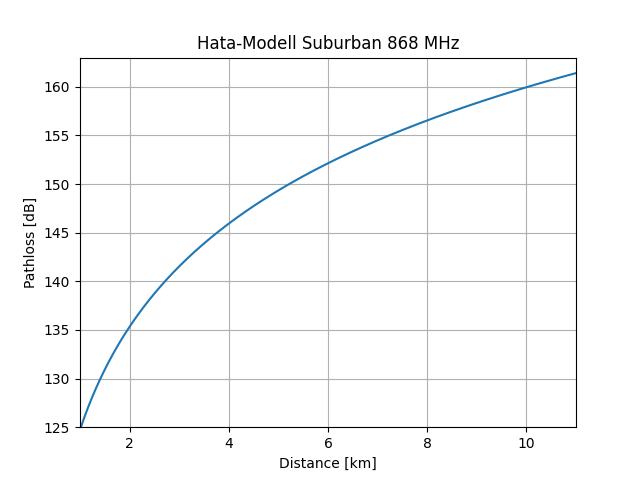
\includegraphics[scale=0.7]{./Bilder/Theorie/Hata_Suburban_868MHz.png}
\end{figure}
Die Grafik zeigt die Reichweite nach dem Okumura-Hata-Modell für ein Suburbanes Gebiet bei Nutzung einer 868MHz frequenz. Wie der Grafik zu entnehmen, wird bei unsererem Linkbudget von 152dBm maximal eine Reichweite von ungefähr 6km möglich\\

Die bereitgestellten Formeln decken nicht alle im Okumura-Modell vorgeschlagenen Bedingungen ab. Hatas Ansatz gilt nur mit folgende Einschränkungen:\\
\\ \\
\begin{tabular}[h]{l | l}
Frequenz  & 150-1500 MHz \\
\hline
Distanz  & 1-20km\\
\hline
Höhe Senderantenne  & 30-200m\\
\hline
Höhe Empfängerantenne & 1-10m \\
\end{tabular} \\ \\ \\
\newpage
\text{Mit folgenden Werten wurde im suburbanen gearbeitet: }\\
\begin{align*}
\\
h_s &= 30\mathrm{m} \\
h_r &= 2\mathrm{m} \\
f &= 869\mathrm{MHz} \\
\\
A &= 69.55 + 26.16 \cdot \log_{10}{(f)} - 13.82 \cdot \log_{10}{(h_s)} \\
&= 69.55 + 26.16 \cdot \log_{10}{(868)} - 13.82 \cdot \log_{10}{(30)} \\
&\thickapprox 126.008 \\
\\
B &= 44.9 - 6.55 \log_{10}{(h_s)} \\
&= 44.9 - 6.55 \log_{10}{(30)}\\
&\thickapprox 35.225\\
\\
K &= (1.1 \cdot log_{10}{(f)} - 0.7) \cdot h_r - (1.56 \cdot \log_{10}{(f)} - 0.8) \\
&= (1.1 \cdot log_{10}{(868)} - 0.7) \cdot 2 - (1.56 \cdot \log_{10}{(868)} - 0.8) \\
&\thickapprox 1.281 \\
\\
C &= 0 \\
\end{align*}
\\
\begin{align*}
Loss(dB) &= A + B \cdot log_{10}{(d)} - K + C \\
log_{10}{(d)} &= \frac{Loss(dB) - A + K - C}{B} \\
d &= 10^\frac{Loss(dB) - A + K - C}{B} \\
&= 10^\frac{Loss(dB) - 126.008 + 1.281 - 0}{35.225}\\
&= 10^\frac{Loss(dB) - 124.727}{35.225}\\
\end{align*}
\newpage

\begin{tabular}[h]{l | l}
Freifläche(Max)  & 64.640km (Begrenzung! Sichtlinie 24.6km) \\
\hline
Suburban(Max) & 10.130km \\
\hline
Urban(Max) & 9.975km\\
\hline
\hline
\hline
Freifläche(152dB) & 37.943km (begrenzt auf Sichtlinie 24.6km) \\
\hline
Suburban(152dB) & 5.946km \\
\hline
Urban(152dB) & 15.855km \\
\hline
\hline
\hline
Freifläche(Gebäude) & 12.612km\\
\hline
Suburban(Gebäude) & 1.220km\\
\hline
Urban(Gebäude) & 1.018km\\
\hline
\hline
\hline
Sichtlinie & 24.6km
\end{tabular} \\ \\
\\
Es darf nicht vergessen werden, dass das Hata-Modell nur eine annäherung im Bereich bei Entfernungen um die 1-20km ist. Alle Werte die darüber berechnet werden sollten mit anderen Werkzeugen überprüft werden. Wie in unserem Fall Freifläche(Max) und Freifläche(Gebäude).\\
  \\
Für (Gebäude) wird eine Dämpfung von 17dB für das Eindringen in Gebäude und ein Verlust von 8dB für das Fading angenommen. Das bedeutet, dass die Analyse an die Bedingungen für Sender innerhalb von Gebäuden angepasst wurde. Das Link-Budget wird daher um 25 dB auf 128dB reduziert.\\
\\
Für (Max) wird das maximal mögliche legale Limit für Sendeleistung und Antennenverstärkung ausgereizt und liegt bei einem Linkbudget, wie anfänglich dargelegt, von 160.15dB.\\
\\
(152dB) beschreibt die maximal mögliche ausbreitung des Signals bei der Sendeleistung der von uns verwendeten Geräte.\\
\\
Die Höhe der Antenne des Senders wurde auf 30Meter festgelegt, da dass Hata Modell nur mit dieser minimalen Höhe arbeiten kann.  \\
Die Empfängerantenne liegt auf 2Meter Höhe.

\subsection{Fazit}

Das Hata-Modell kennt keine Erdkrümmung und ist nur eine erste Näherung. Als Kontrolle sollten bei Berechnungen immer die Sichtlinie beachtet werden und damit die plausabilität der Berechnung kontolliert und ggf. eingeschränkt werden. Die minimale Höhe der Senderantenne macht die Anwendung des Hata-Modells für unser Projekt weniger praktikabel gibt jedoch einen ersten Anhaltspunkt um mit unseren Messwerten zu vergleichen.
\newpage
\subsection{Notizen}
\subsubsection{Link-Budget Formel}
\begin{align*}
PRX &= PTX + GTX + GRX - LTX - LFS - LP - LRX \\
PRX &= \text{received power (dBm)} \\
PTX &= \text{transmitter output power (dBm)} \\
GTX &= \text{transmitter antenna gain (dBi)} \\
GRX &= \text{receiver antenna gain (dBi)} \\
LTX &= \text{transmit feeder and associated losses (feeder, connectors, etc.) (dB)} \\
LFS &= \text{free space loss or path loss (dB)} \\
LP  &= \text{miscellaneous signal propagation losses} \\
    &\phantom{=} \text{(these include fading margin, polarization mismatch, losses associated with} \\
   &\phantom{=} \text{medium through which signal is travelling, other losses...) (dB)} \\
LRX &= \text{receiver feeder and associated losses (feeder, connectors, etc.) (d)B} \\
\\
\\
FSPL \mathrm{(dB)} &= 20\log_{10}(d) + 20\log_{10}(f) - 147.55 \\
FSPL &= (4\pi d/ \lambda) \cdot 2 = (4\pi df/c) \cdot 2 \\
FSPL &= \text{Free Space Path Loss (Freiraumdämpfung)} \\
d &= \text{Abstand zwischen Tx und Rx in Metern} \\
f &= \text{Frequenz in Hertz} \\
\\
\text{Rx-Empf.} &= -174 + 10\log_{10}(BW) + NF + SNR \\
BW &= \text{Bandbreite in Hz} \\
NF &= \text{Rauschfaktor in dB} \\
SNR &= \text{Signal-Rausch-Verhältnis (signal to noise ratio).} \\
    &\phantom{=} \text{Es gibt an, wie weit das Signal über dem Rauschen liegen muss.}\\
\end{align*}

\subsubsection{Line of Sight tool}

\url{https://www.heywhatsthat.com}
\newpage
\subsubsection{Beispielrechnung}

Let's consider a simplified example of a LoRa link budget for a point-to-point communication link. Please note that real-world scenarios are more complex and involve additional factors, but this example should provide a basic understanding:

1. \textbf{Transmit Power (Tx Power):} Let's assume the transmitter has a power output of 20 dBm.

2. \textbf{Frequency (f):} Assume a frequency of 868 MHz.

3. \textbf{Distance (d):} Let's consider a communication distance of 2 kilometers.

4. \textbf{Antenna Gains (Gt and Gr):} Assume both the transmitter and receiver antennas have a gain of 2 dBi.

5. \textbf{Free Space Path Loss (Lp):} Using the free space path loss formula:

   $$
   Lp = 20 \log_{10}{d} + 20 \log_{10}{(f)} + L_{FS}
   $$

   $$
   Lp = 20 \log_{10}{2} + 20 \log_{10}{(868 \cdot 10^6)} + 20 \cdot \log_{10}{\frac{4\pi}{c}}
   $$

   Here, \(c\) is the speed of light. The result will be the path loss in dB.

6. \textbf{Received Power (Rx Power):} Plug the values into the link budget equation:

   $$
   \text{Rx Power} = \text{Tx Power} + \text{Tx Antenna Gain} - \text{Path Loss} + \text{Rx Antenna Gain}
   $$

   Substitute the values and calculate the received power.

The calculated received power should be compared with the receiver's sensitivity specification. If the received power is higher than the sensitivity threshold, the link is expected to work under the specified conditions.

Keep in mind that this is a simplified example, and in a real-world scenario, additional factors such as atmospheric conditions, interference, and fading effects should be considered for a more accurate link budget analysis.
\newpage
\section{Fazit}
Meshtastic ist ein gut voranschreitendes Projekt, dass eine solide Software-Plattform für die Kommunikation
zwischen LoRa-fähigen Geräten ermöglicht.\\
\\
Damit aber Meshtastic als Katastrophennetz eingesetzt werden könnte, sind aktuell noch einige Hürden im Weg.\\
\\
Für den Einsatz als Katastrophennetz müssten erstmal genug solcher Meshtastic- und LoRa-fähigen Geräte angeschafft werden,
sodass ein zuverlässiges Mesh-Netzwerk innerhalb der Stadt aufgebaut werden könnte. Dies müsste am Besten mit einer Großbestellung geschehen,
da sonst der Markt überlastet werden und die Preise steigen könnten.\\
\\
Es müssten genug Geräte innerhalb der Stadt hoch positioniert werden, da die Reichweite von LoRa durch Gebäude wesentlich begrenzt ist.
Nur bei freier Luftlinie sind Verbindungen über mehrere Kilometer möglich. Andere Funktechnologien mit mehr Sendeleistung, sind
durch Gebäude weniger beeinträchtigt.
Aber im Katastrophenfall mit zusammengebrochener Infrastruktur (Black-Out), ist LoRa mit geringem Energieverbrauch besser geeignet.\\
\\
Aktuell ist Meshtastic noch softwareseitig auf Netzwerke mit bis zu 80 Nodes limitiert. Das reicht bei Weitem nicht, um den Raum Dresden
vollständig abzudecken.
Das Protokoll scheint auch nicht für solche Mega-Meshes ausgelegt zu sein, was man am maximalen Hop Count von 7 erkennen kann.
Ein limitierter Hop Count könnte eine weitreichende Zustellung verhindern.\\
\\
Die Software ist für ein Open Source Projekt ohne große Finanzierung auf einem guten Niveau,
aber noch nicht für allgemeine Nutzung ausgereift. Dafür würde es einen Feinschliff in User Experience und Stabilität benötigen.\\
\end{document}
